
\documentclass[11pt]{article}
\usepackage{UF_FRED_paper_style}
\usepackage{listings}
\usepackage{hyperref}
\hypersetup{
	colorlinks=true,
	linkcolor=blue,
	filecolor=blue,      
	urlcolor=blue,
	citecolor=cyan,
}

%% ===============================================
%% Setting the line spacing (3 options: only pick one)
% \doublespacing
% \singlespacing
\onehalfspacing
%% ===============================================

\setlength{\droptitle}{-5em} %% Don't touch

% %%%%%%%%%%%%%%%%%%%%%%%%%%%%%%%%%%%%%%%%%%%%%%%%%%%%%%%%%%
% SET THE TITLE
% %%%%%%%%%%%%%%%%%%%%%%%%%%%%%%%%%%%%%%%%%%%%%%%%%%%%%%%%%%

% TITLE:
\title{COMSM0104: Web Technologies 2019 \\Final Assignment Report}

% AUTHORS:
\author{Tao Xu\\% Name author
	\href{mailto:si19010@bristol.ac.uk}{\texttt{si19010@bristol.ac.uk}} %% Email author 1 
	\and Yinan Yang\\% Name author
	\href{mailto:ff19085@bristol.ac.uk}{\texttt{ff19085@bristol.ac.uk}} %% Email author 2
}

% DATE:
\date{\today}
% %%%%%%%%%%%%%%%%%%%%%%%%%%%%%%%%%%%%%%%%%%%%%%%%%%%%%%%%%%
% %%%%%%%%%%%%%%%%%%%%%%%%%%%%%%%%%%%%%%%%%%%%%%%%%%%%%%%%%%
\begin{document}

	% %%%%%%%%%%%%%%%%%%%%%%%%%%%%%%%%%%%%%%%%%%%%%%%%%%%%%%%%%%
	% %%%%%%%%%%%%%%%%%%%%%%%%%%%%%%%%%%%%%%%%%%%%%%%%%%%%%%%%%%
	% ABSTRACT
	% %%%%%%%%%%%%%%%%%%%%%%%%%%%%%%%%%%%%%%%%%%%%%%%%%%%%%%%%%%
	% %%%%%%%%%%%%%%%%%%%%%%%%%%%%%%%%%%%%%%%%%%%%%%%%%%%%%%%%%%
	{\setstretch{.8}
		\maketitle
		% %%%%%%%%%%%%%%%%%%
		\begin{abstract}
			% CONTENT OF ABS HERE--------------------------------------
			
			Our team consists of Tao Xu (si19010) and Yinan Yang (ff19085). Due to the impact of Covid19, we collaboarated remotely via GitHub to co-develop this project.
			
			Our website is an online CV maker, featuring a simple and convenient interface for editing, online storage (at our server) and extensibility (the CV templates are easy to make).
			
			The frontend of our website was based on the Vue framework, taking advantage of Vue's MVVM, the Model-View-View Model, which helped us in keeping code modular and implementing reactive user interfaces.
			
			The backend of our website was powered by Node.js with Express.js and SQLite.
			
			
			% END CONTENT ABS------------------------------------------
			\noindent
			\textit{\textbf{Keywords: }%
				Vue, Node-Js, SQLite.} \\ %% <-- Keywords HERE!
			\noindent
			% \textit{\textbf{JEL Classification: }%
			% Q12; C22; D81.} %% <-- JEL code HERE!
			
		\end{abstract}
	}
	
	% %%%%%%%%%%%%%%%%%%%%%%%%%%%%%%%%%%%%%%%%%%%%%%%%%%%%%%%%%%
	% %%%%%%%%%%%%%%%%%%%%%%%%%%%%%%%%%%%%%%%%%%%%%%%%%%%%%%%%%%
	% BODY OF THE DOCUMENT
	% %%%%%%%%%%%%%%%%%%%%%%%%%%%%%%%%%%%%%%%%%%%%%%%%%%%%%%%%%%
	% %%%%%%%%%%%%%%%%%%%%%%%%%%%%%%%%%%%%%%%%%%%%%%%%%%%%%%%%%%
\begin{spacing}{1.0}
	\tableofcontents
	\newpage	
	% --------------------
	\section{Introduction}
	% --------------------
	
	\hspace{\parindent}The website we created, named "Simple Resume Maker", was an online CV maker, where users could employ the CV templates provided by us to make tailored resumes of their own. 
	
	Basic editing features like text editing, adding/removing pages, inserting/deleting sections, italicising/boldifing text, increasing/decreasing font size, and uploading avatar have been implemented in the frontend. Users could also save and load their progress and generate their CVs in pdf format, these features are powered by the backend.
	
	In short, the idea behind our CV-maker was that the contents of a CV was just the plain html in the container enclosing the CV pages, and how the CV was displayed were only affected by the CSS code applied, which were present in the "\textless head\textgreater" section of the document. Therefore, when saving and loading the progress, the "\textless head\textgreater" and the "\textless div\textgreater" containing the CV contents were uploaded to and downloaded from our server, respectively. Applying different templates was actually just replacing one CSS file that was being used with another, which also made our templates quite easy to make since they were just CSS files. When a user requests to download a pdf version of their CV, the backend loads their data from the database and creates a temporary html file that contains all the information needed to regenerate the CV pages that the user sees. This temporary html is then loaded by the "puppeteer" module at our server, which is a headless Chrome browser. So the temporary html page should appear exactly the same as the related section of the page that the user sees (if the user is using a Chrome browser or other browsers that have the same behaviour as chrome). The "puppeteer" module then convert the page into pdf, which will be related by our server to the user.
	
	Logging in is required for users to access any information regarding CV contents stored at the backend, including avatars and text. After logging in, each user is assigned an encryped JSON web token (JWT) containing their user Id. This JWT is stored as a Cookie so that it will be present in every request to the server from the user thereafter. Our server identifies users by verifying the JWTs and reading the user Id information from the JWTs. Therefore, as long as a user do not leak the JWT, no one else could access their data, which protects the users' privacy to some extent.
	
	Although our website does not provides extensive functionalities regarding text editing compared to mainstream text editors, our aim was to give users experience of editing documents online. Moreover, what would otherwise be a cumbersome formatting process was made easier with employing different CSS code. This addresses the initial point we made in designing the product, which was to make things easier.
	
	In building this site, we used the VUE framework, which is a progressive framework for building user interfaces. 
	
	\begin{center}
		\fbox{\shortstack[l]{
				Unlike other monolithic frameworks, Vue is designed from the ground up to be\\ incrementally adoptable. The core library is focused on the view layer only, and\\ is easy to pick up and integrate with other libraries or existing projects. On the\\ other hand, Vue is also perfectly capable of powering sophisticated Single-Page\\ Applications when used in combination with modern tooling and supporting\\ libraries.\\
				----- Official development documentation from Vue
			}}
		
	\end{center}

	
	\subsection{Set up the environment}
	\hspace{\parindent}\hspace*{1cm}npm install
	\subsection{Compile the frontend}
	\hspace{\parindent}\hspace*{1cm}npm run build
	\subsection{Run the server}
	\begin{itemize}
  		\item localhost https (recommended):\\
  		\hspace*{1cm} node server.js
  		\item cloud https:\\
  		\hspace*{1cm} node server.js -cloud
  		\item http only:\\
  		\hspace*{1cm} node server.js -http
  		\item query the database:\\
  		\hspace*{1cm} node server.js -sql
	\end{itemize}

	\subsection{NOTE}
	For the server-side node module "puppeteer" to function, you may need to install some dependencies if you don't have:
	\href{https://github.com/puppeteer/puppeteer/blob/master/docs/troubleshooting.md#chrome-headless-doesnt-launch-on-unix%20dependencies}{Puppeteer dependencies}.
	Otherwise, the pdf generator may not work, although it won't crash the server.
		
	% --------------------
	\section{Self Evalutation}
	\subsection{Estimation of marks}
\begin{itemize}
	\item A+ for HTML
	\item A for CSS
	\item A for JS
	\item A for PNG	
	\item A for SVG
	\item A for Server
	\item A for Database
	\item A for Dynamic pages
\end{itemize}
	\subsection{Client Side}
	\subsubsection{HTML}
	\begin{itemize}
  		\item We have been quite proficient in generating HTML pages via the Vue framework. \\

	\hspace{\parindent}In terms of front-end technology, we utilised the Vue architecture, with Vue-CLI aiding our development. We chose Vue because we wanted to develop a less web-heavy application, which is the trend in some part of the world. Had we used React, it might have been the right choice at some point, but the frontend pages as a whole would have been weighty and heavily dependent on communications to and from the backend, which would have been a departure from our original intent.
	
	\hspace{\parindent}The Vue-router facilitates routing at the frontend, which reduces the burden of the server.
The Vue compiler compiles and compresses a project into a single page website, where all the HTML contents are injected to that page at run-time, which reduces the overall size of a website. 
	If you visit our website, you will see that while it appears like there are multiple pages, there is actually only one page with dynamically changing contents, which is achieved with the power of the Vue-router:
	\begin{figure}[H]
	\centering
	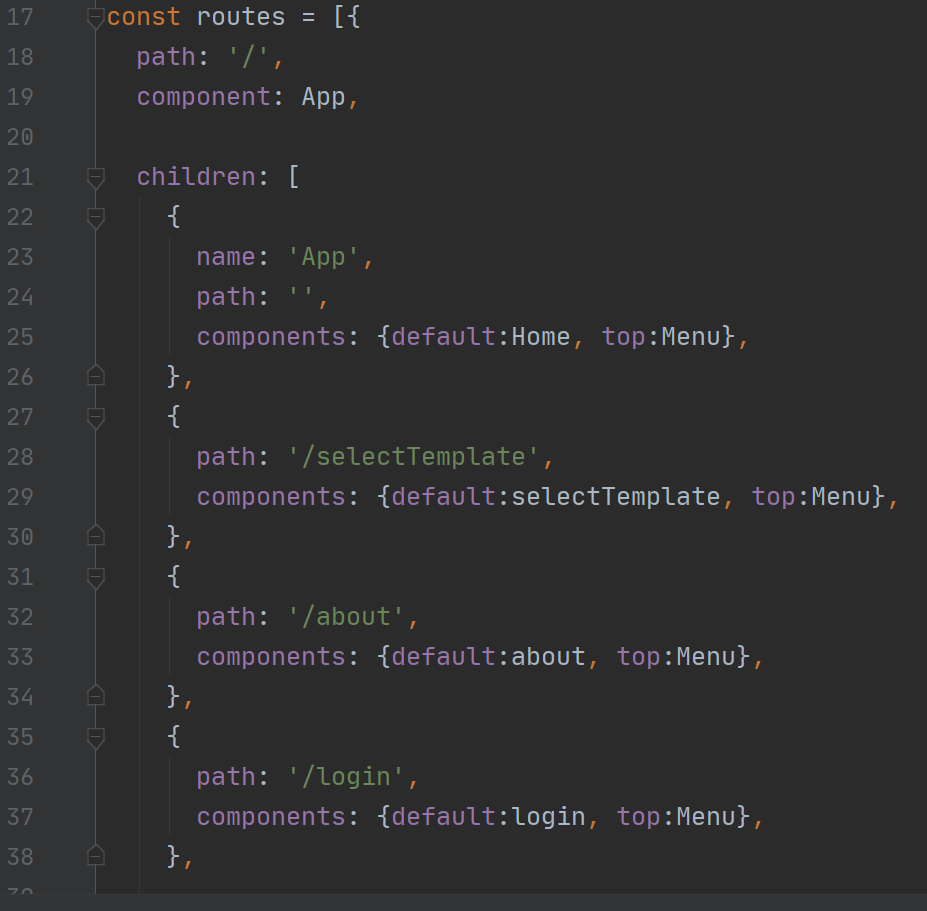
\includegraphics[scale=.3]{figures/routes.png}
	\caption{routes}
	\label{fig:8}
\end{figure}
	
	We completed a total of more than 30 Vue components with multiple levels of parent-child relationships, and they worked quite perfectly. Thanks to Vue's component-based design model, our front-end application is not as messy as what it would have been a decade ago. Moreover, this design pattern will make maintenance in the future  quite effortless.
	\begin{figure}[H]
		\centering
		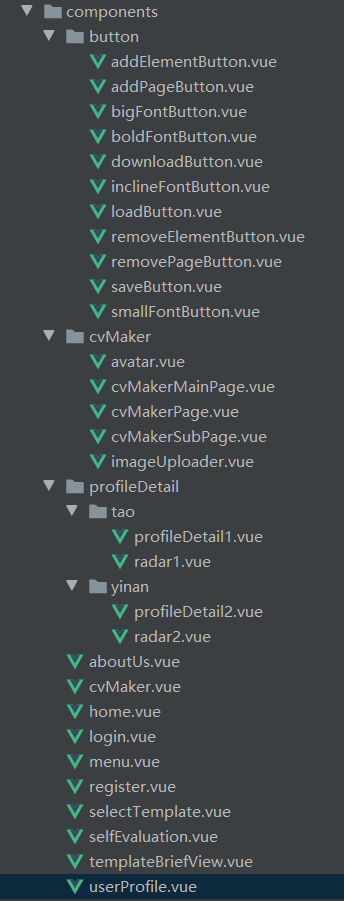
\includegraphics[scale=.5]{figures/components.png}
		\caption{components}
		\label{fig:7}
	\end{figure}

	Below is an example of multi-level hierarchy, where the "cvMakerPage" has two children components: "mainPage" and "subPage", which will never be visible at the same time, while the "mainPage" has a child "avatar". Furthermore, the "avatar" has a child "imageUploader":
	\begin{figure}[H]
	\centering
	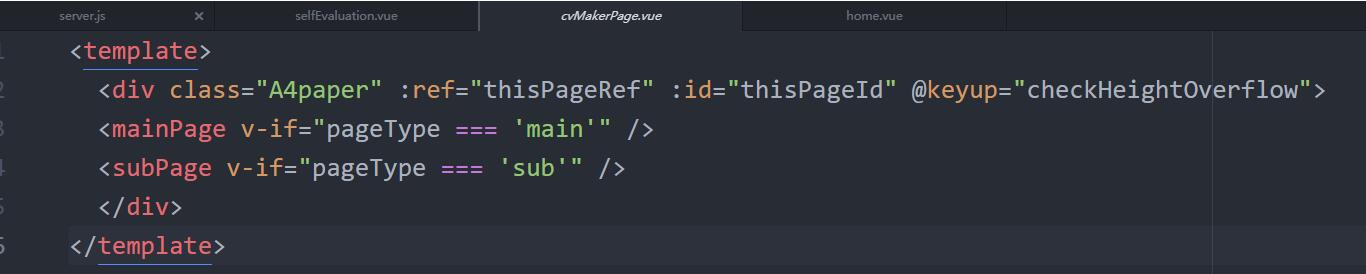
\includegraphics[scale=.3]{figures/html/2_cvMakerPage.jpg}
	\caption{cvMakerPage}
	\end{figure}
	
	\begin{figure}[H]
	\centering
	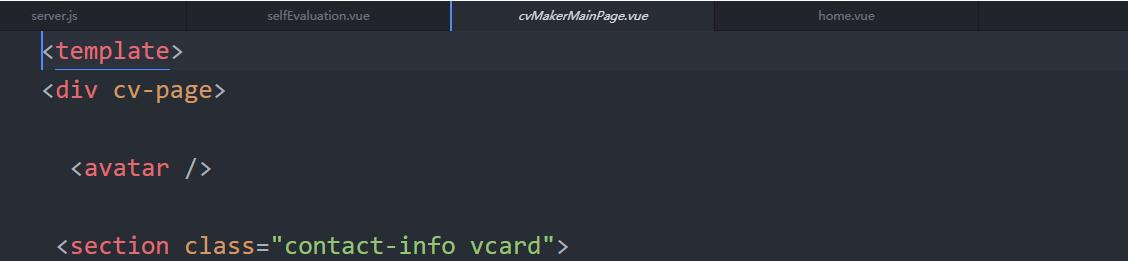
\includegraphics[scale=.4]{figures/html/2_cvMakerMainPage.jpg}
	\caption{mainPage}
	\end{figure}
	
	\begin{figure}[H]
	\centering
	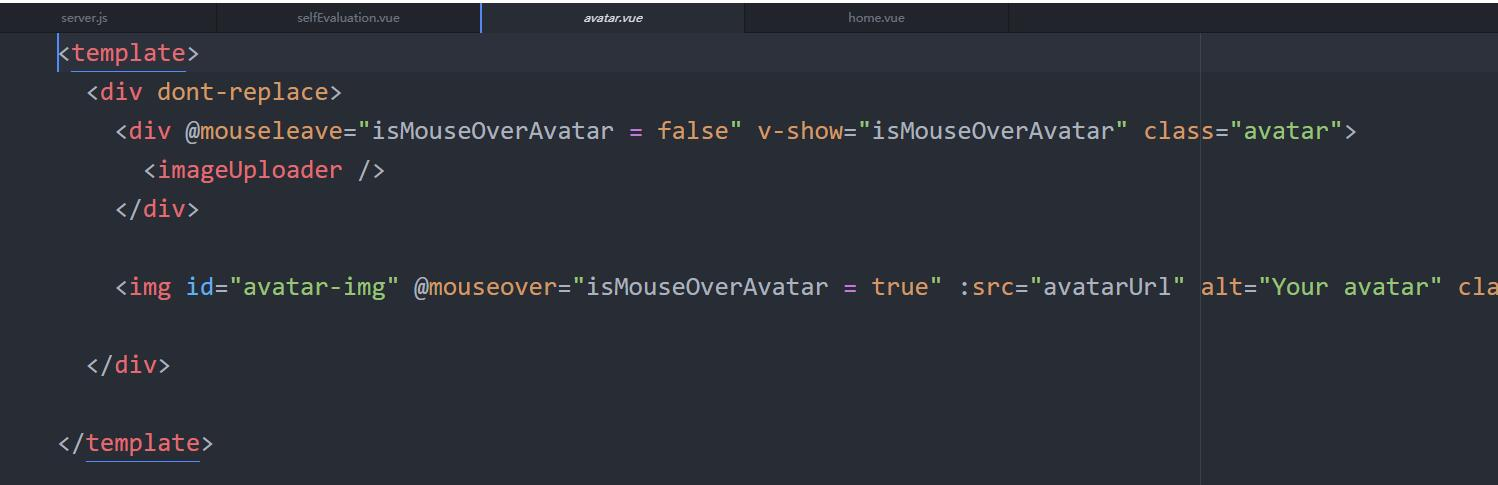
\includegraphics[scale=.3]{figures/html/2_avatar.jpg}
	\caption{avatar}
	\end{figure}


	\item The main functionality of our website is online CV making, which was implemented by editing the html. Without decent understanding about the HTML, we wouldn’t have made it functioning.
	For example, the italicising, boldifing and font size increasing/decreasing functionalities were implemented by inserting "i", "b", "larger", "smaller" tags around the text that users select, respectively:
	\begin{figure}[H]
	\centering
	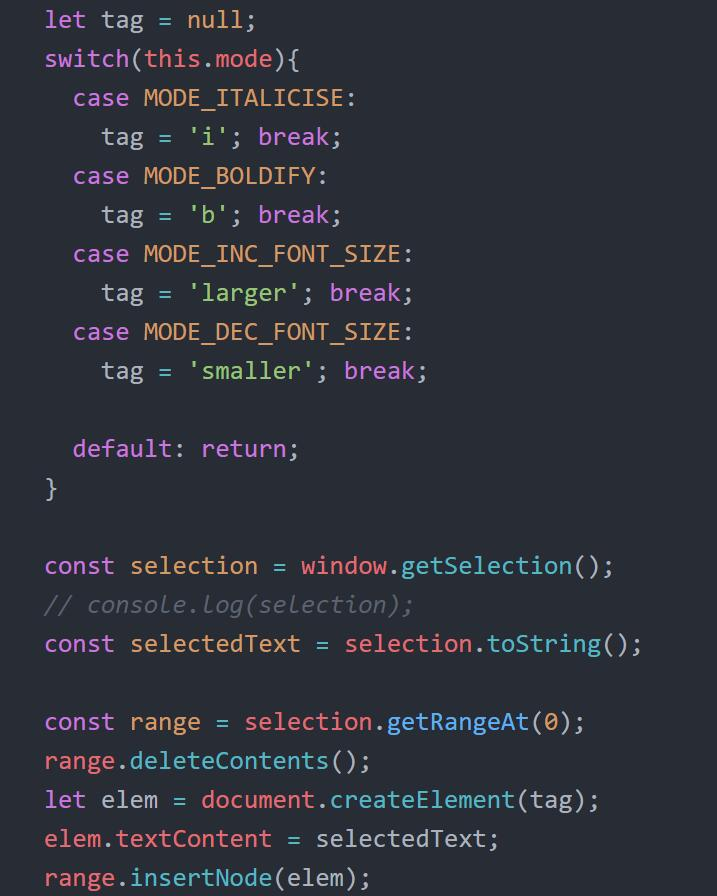
\includegraphics[scale=.5]{figures/html/3_insertTag.jpg}
	\caption{Inserting tags}
	\end{figure}
		
	We explored many HTML features such as contenteditable, which powered the text-editing functionality of the CV pages, and custom attributes, which we used to distinguish something that should be treated differently from their siblings.
	
	As the above Fig.5 avatar shows, the first div has a custom attribute "dont-replace", because we do not want it to be replaced during loading progress. And this information is captured in the "loadSavedData" method of the cvMaker.vue component:
	\begin{figure}[H]
	\centering
	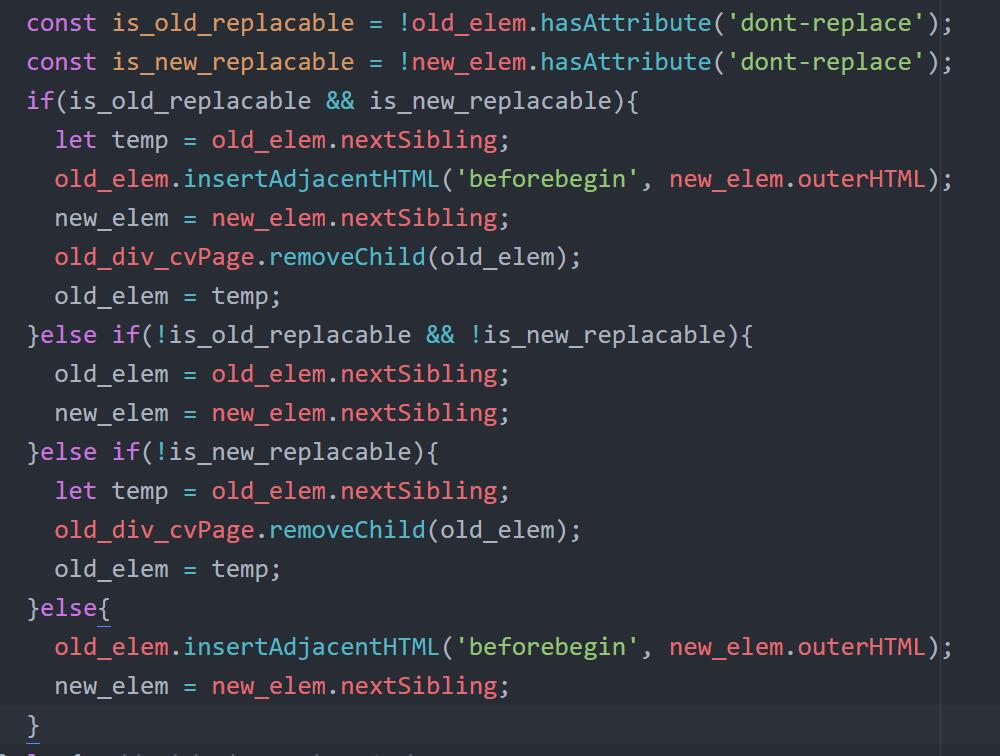
\includegraphics[scale=.5]{figures/html/3_customAttr.jpg}
	\caption{custom attribute}
	\end{figure}
	
	\item I think the idea behind our project, i.e. employing HTML and CSS and their manipulation to make text editors with built-in templates is quite innovative and creative, and we came up with it by ourselves, which I think might worth some meagre credit. That is why I am so arrogantly claiming an A+. 
	
	\end{itemize}
	\subsubsection{CSS}
	\begin{itemize}
	\item
	We used the Vue framework to deliver pages, so it’s quite difficult to tell whether we had “style” tag in HTML pages because we did not have HTML pages during development. The styles resided in the “style” section for each Vue file and they were injected into the $<head>$ part of the page as $<style>$ tags at runtime. It’s just how the framework worked.
However, we made sure we didn’t have style attributes in the template section of Vue files.
	\item
	Each Vue file could have any number of "style" tags to contain CSS code, which already satisfies the purpose of not having internal or inline CSS code in traditional website, that is to keep different things at different places so that everything is more modular and therefore easier to maintain. The CSS code in Vue files are already separate from HTML as long as we do not put them in the "template" section, and we did not. Despite that, we still placed most CSS code in separate files under the folder $src/view/index/assets$ for easier management.

	\item
	We successfully used basic CSS, Vue specific CSS and the classes provided by the Bootstrap framwork to make our frontend pages satisfy our poor and abnormal aesthetics. 
	
	Vue has two options for CSS code positioned in the "style" section: global or scoped. Although they will both be injected to the "head" section of the page when the pages are rendered, scoped CSS will have a "data-?" attribute attached to them, where ? is a seemly random value but is resolved at compile time. All the tags that related to a scoped CSS will be added the same attribute as the CSS. That is how the Vue identifies them.
	
	Scoped CSS with combined or descendant selectors were used for precise location in specific pages while global class like .background (one with a furry glass effect to give the whole screen more colour) is accessible from all the pages.
	
	Below is an example of using Vue specific CSS (the deep selector $>>>$):
	\begin{figure}[H]
	\centering
	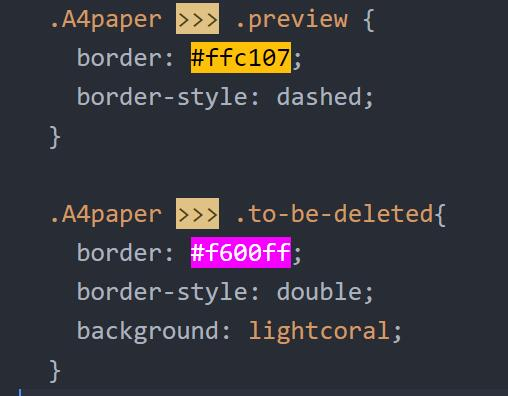
\includegraphics[scale=.5]{figures/html/4_basicCSS.jpg}
	\caption{Vue CSS}
	\end{figure}

	,which means every item that has class "preview" inside a container with class "A4paper" will have a yellow dashed border even those that are rendered by child components. Similarly, every item that has class "to-be-deleted" inside a "A4paper" container will have a red-purplish double border and a lightcoral background. In insertion/deletion mode of the CVmaker page, these two classes are added to the item that the user's mouse cursor is currently pointing at, and removed from that item when the cursor moves away. 
	

		\item 
		The following is an example of how to adjust the progress bar according to the download progress in the downloadButton. We dynamically adjust the width of the bar to match the expected download time. By the way, a timer was used to control how often the progress bar refreshed to avoid blocking the execution since javascript is single-threaded.
\begin{figure}[H]
	\centering
	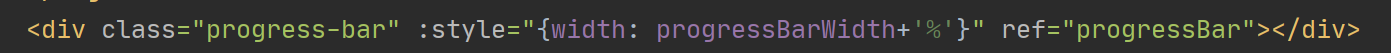
\includegraphics[scale=.5]{figures/css.png}
	\caption{change style}
	\label{fig:10}
\end{figure}

\item SVG-based animation\\
 We completed some svg-based animation in CSS, which will be explained further in detail in the SVG section.
 \begin{figure}[H]
 	\centering
 	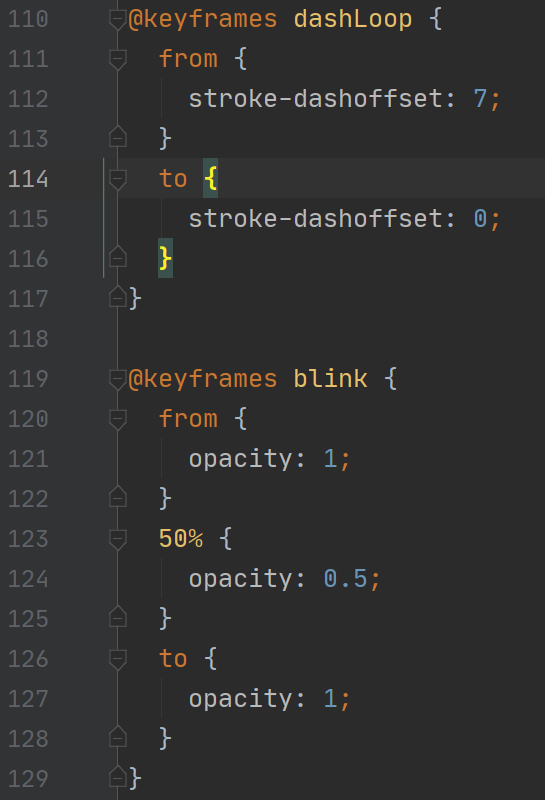
\includegraphics[scale=.5]{figures/cssAnimation2.png}
 	\caption{css animation}
 	\label{fig:11}
 \end{figure}
\item Dynamically retrieving CSS from the server\\
The main feature of our website, i.e. making CVs with different templates is facilitated by dynamically fetching and replacing stylesheets at run-time.  
In CVMaker, the CSS that is responsible for the CV pages are fetched from the server according to the user's choice. Below is the method we wrote to remove existing template(s) and fetch the template that the user choose from the server. To be honest, this method does not fetch the template, it just adds a link to the template to the "head" of the page. 
 \begin{figure}[H]
	\centering
	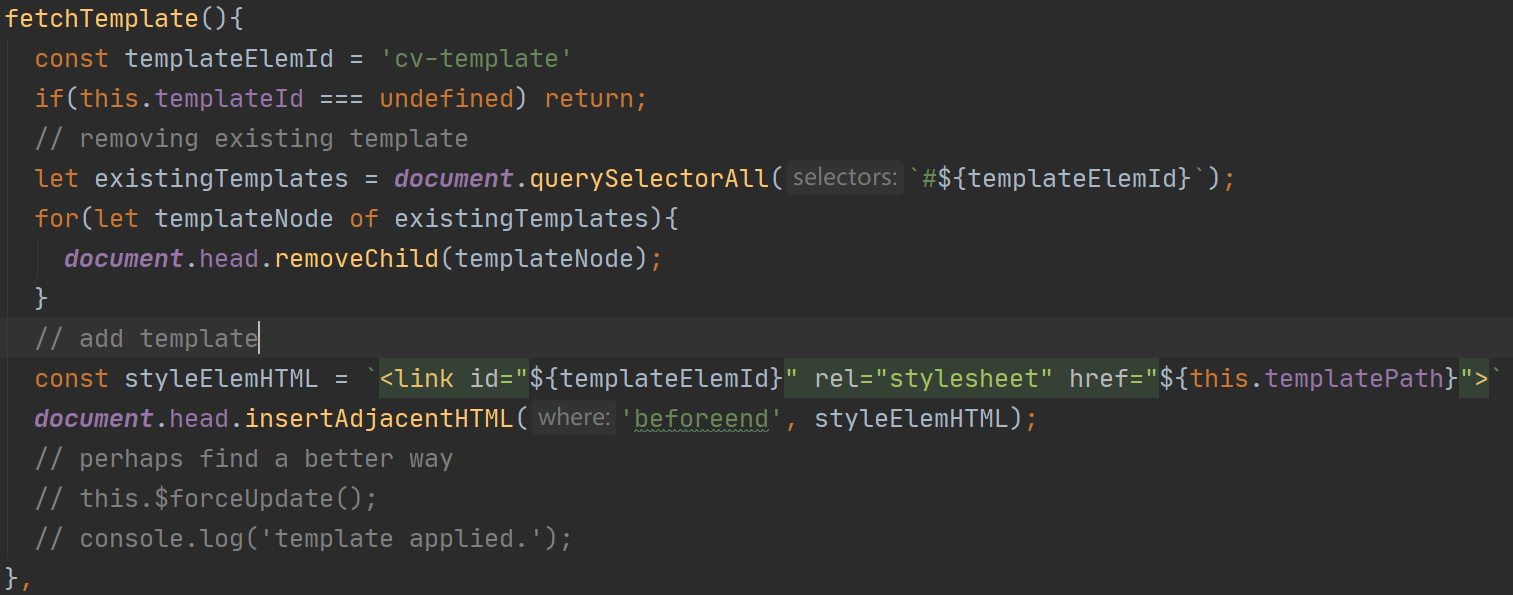
\includegraphics[scale=.4]{figures/cssTemplate.png}
	\caption{fetch template}
	\label{fig:12}
\end{figure}

	\item
	Again, I think using CSS files as templates is quite a good innovation since they are stylesheets themselves but we use them for other purposes rather than just for the sake of beautifying web pages. Furthermore, this also makes our templates quite easy to make: creating a new template is just a matter of creating a new CSS file, which makes our application quite extensible.
		
		
	\end{itemize}
	\subsubsection{JS}We have written a substantial amount of vanilla and Vue-specific javascript code and have implemented all the features we intended. Here we will only discuss some of the code we have written to demonstrate our understanding. 
	\begin{itemize}
	\item DOM manipulation
	
	\begin{figure}[H]
	\centering
	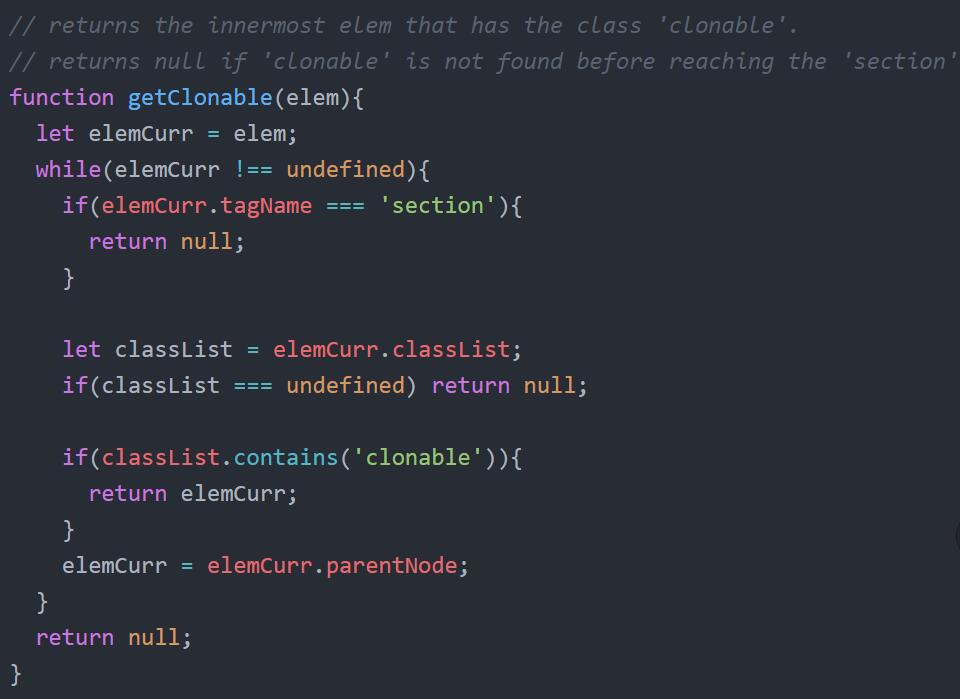
\includegraphics[scale=.5]{figures/js/getClonable.jpg}
	\caption{getClonable()}
\end{figure}

\begin{figure}[H]
	\centering
	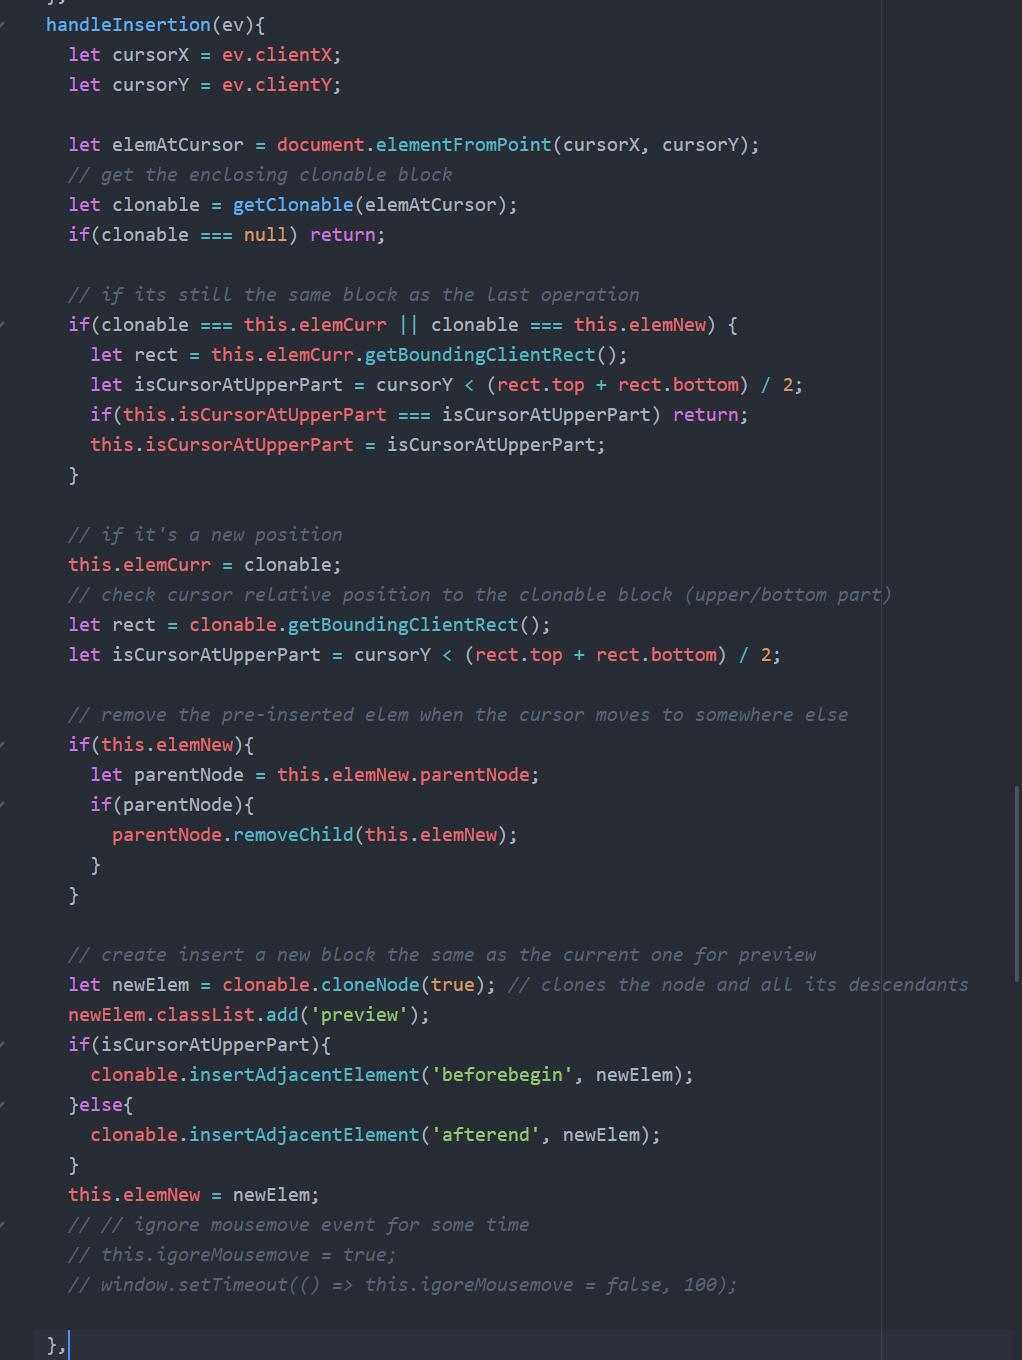
\includegraphics[scale=.5]{figures/js/handleInsertion.jpg}
	\caption{handleInsertion()}
\end{figure}
	The function getClonable and the method handleInsertion are resposible for the "add element" functionality in the CVMaker page. When a mousemove event is triggered and the CVMaker is in the right mode, the event is passed to the handleInsertion method. The method then finds the element that the user's mouse cursor is currently pointing at, checks whether the element is contained in a container with class "clonable". If so, then checks whether the clonable container was created in the previous events or if it is a new target. If it is a new target, the clonable container is cloned and the newly created copy is added a class "preview" for visual effects, then it is inserted before or after the clonable container that was cloned if the cursor is at the upper half or lower half of the container, respectively.
	
	\item HTTP request and save file
	\begin{figure}[H]
	\centering
	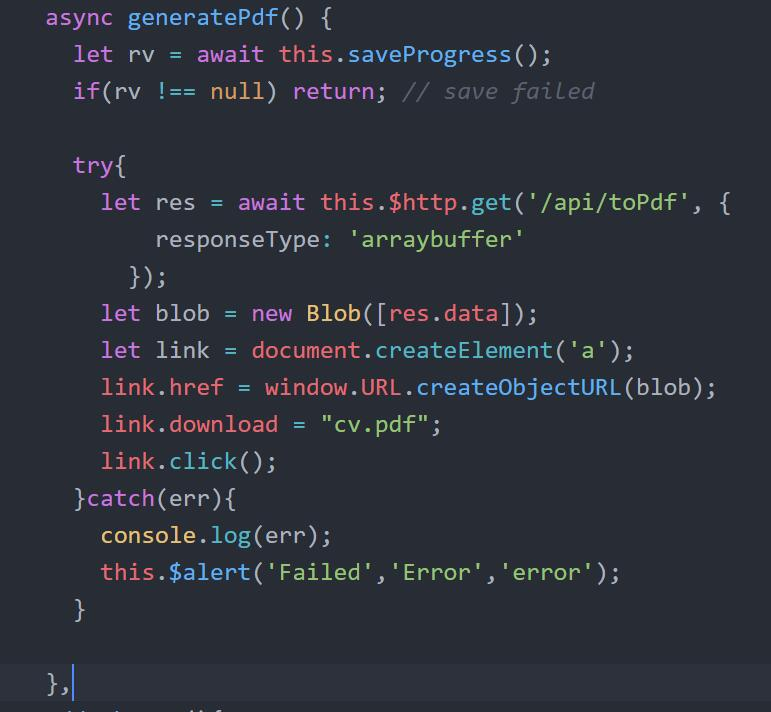
\includegraphics[scale=.5]{figures/js/generatePdf.jpg}
	\caption{handleInsertion()}
\end{figure}

	\item Components communication via Vue reference
	\begin{figure}[H]
	\centering
	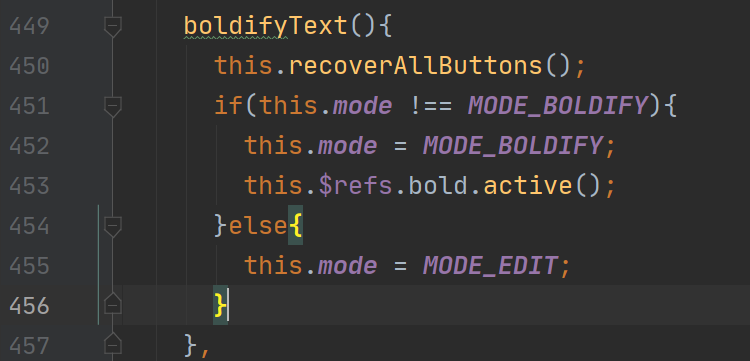
\includegraphics[scale=.5]{figures/componentsRefs.png}
	\caption{component communication}
\end{figure}
	
	
	Above is an example of a parent component calling a child component method. In the CVMaker page, when we press the boldify button in the tools bar, the "active" method of the button will be called.
	
		\item Components communication via event bus
	\begin{figure}[H]
	\centering
	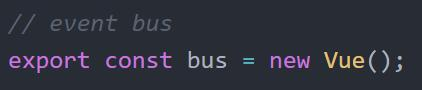
\includegraphics[scale=.5]{figures/js/evbus.jpg}
	\caption{event bus}
\end{figure}		
		
	\begin{figure}[H]
	\centering
	
\includegraphics[scale=.5]{figures/js/event bus.jpg}
	\caption{event bus}
\end{figure}
	An event bus is just another Vue instance. If imported, all the components that have access to it could use it to communicate.
	
	Here is an example of using event bus. The menu bar listens to "getLoginStatus" event. If the event occurs, the menu bar emits another event called "loginStatus" to the bus, passing the login status as a parameter to the potential event handler:
	
	\begin{figure}[H]
	\centering
	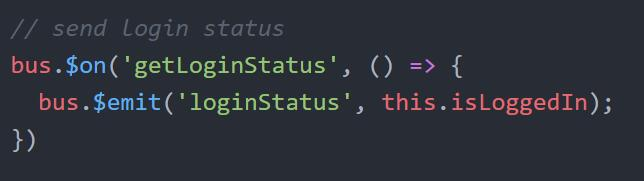
\includegraphics[scale=.5]{figures/js/getLoginStatus.jpg}
	\caption{getLoginStatus}
\end{figure}
	
	Here in userProfile.vue, the method "getLoginStatus" emits a "getLoginStatus" event to the bus. After the menu bar responded, the login status will be stored in the variable "isLoggedIn".
	\begin{figure}[H]
	\centering
	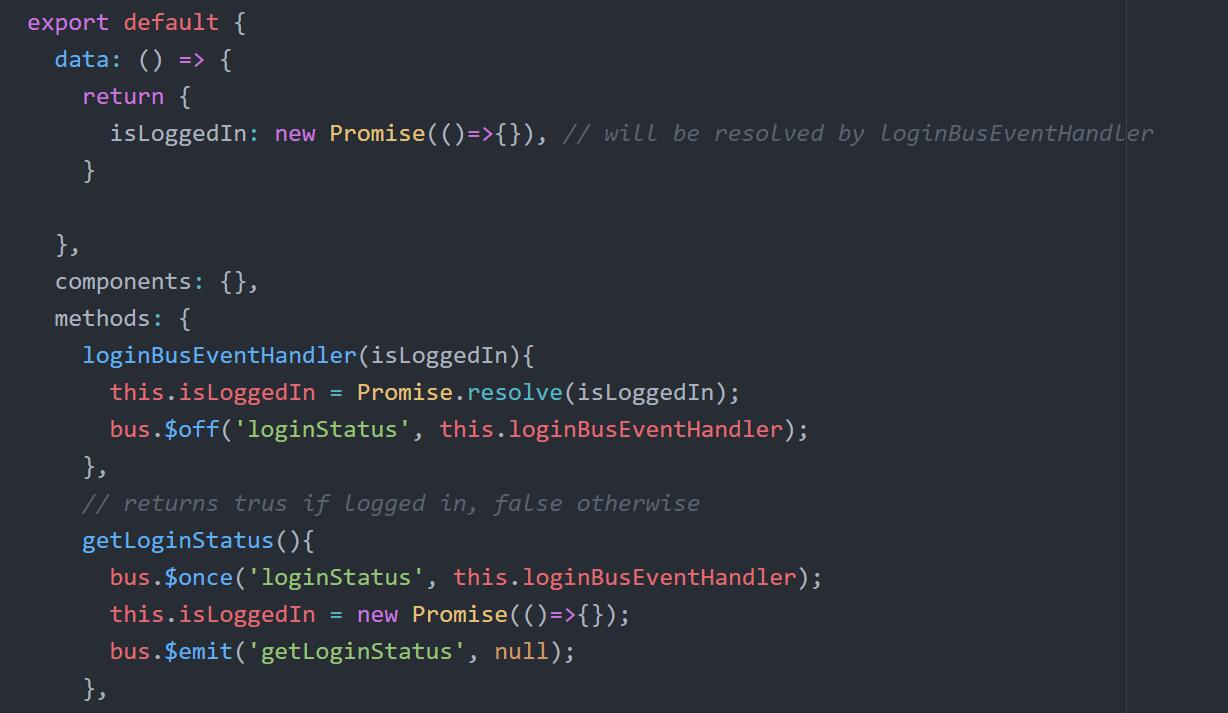
\includegraphics[scale=.5]{figures/js/userpr.jpg}
	\caption{getLoginStatus()}
\end{figure}	
	
	
Here we used Promise because we wanted to make sure the data was available before we used it. Any method that needs to get the login status could then just await the Promise to be resolved, which guarantees the data to be available:
	\begin{figure}[H]
	\centering
	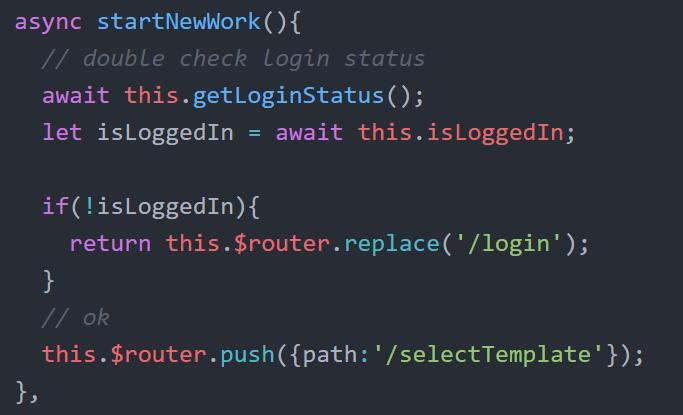
\includegraphics[scale=.5]{figures/js/startNewWork.jpg}
	\caption{startNewWork}
\end{figure}



	
	
	\item Animation\\
	The example below is the method in charge of animating the download button after press:
	 \begin{figure}[H]
		\centering
		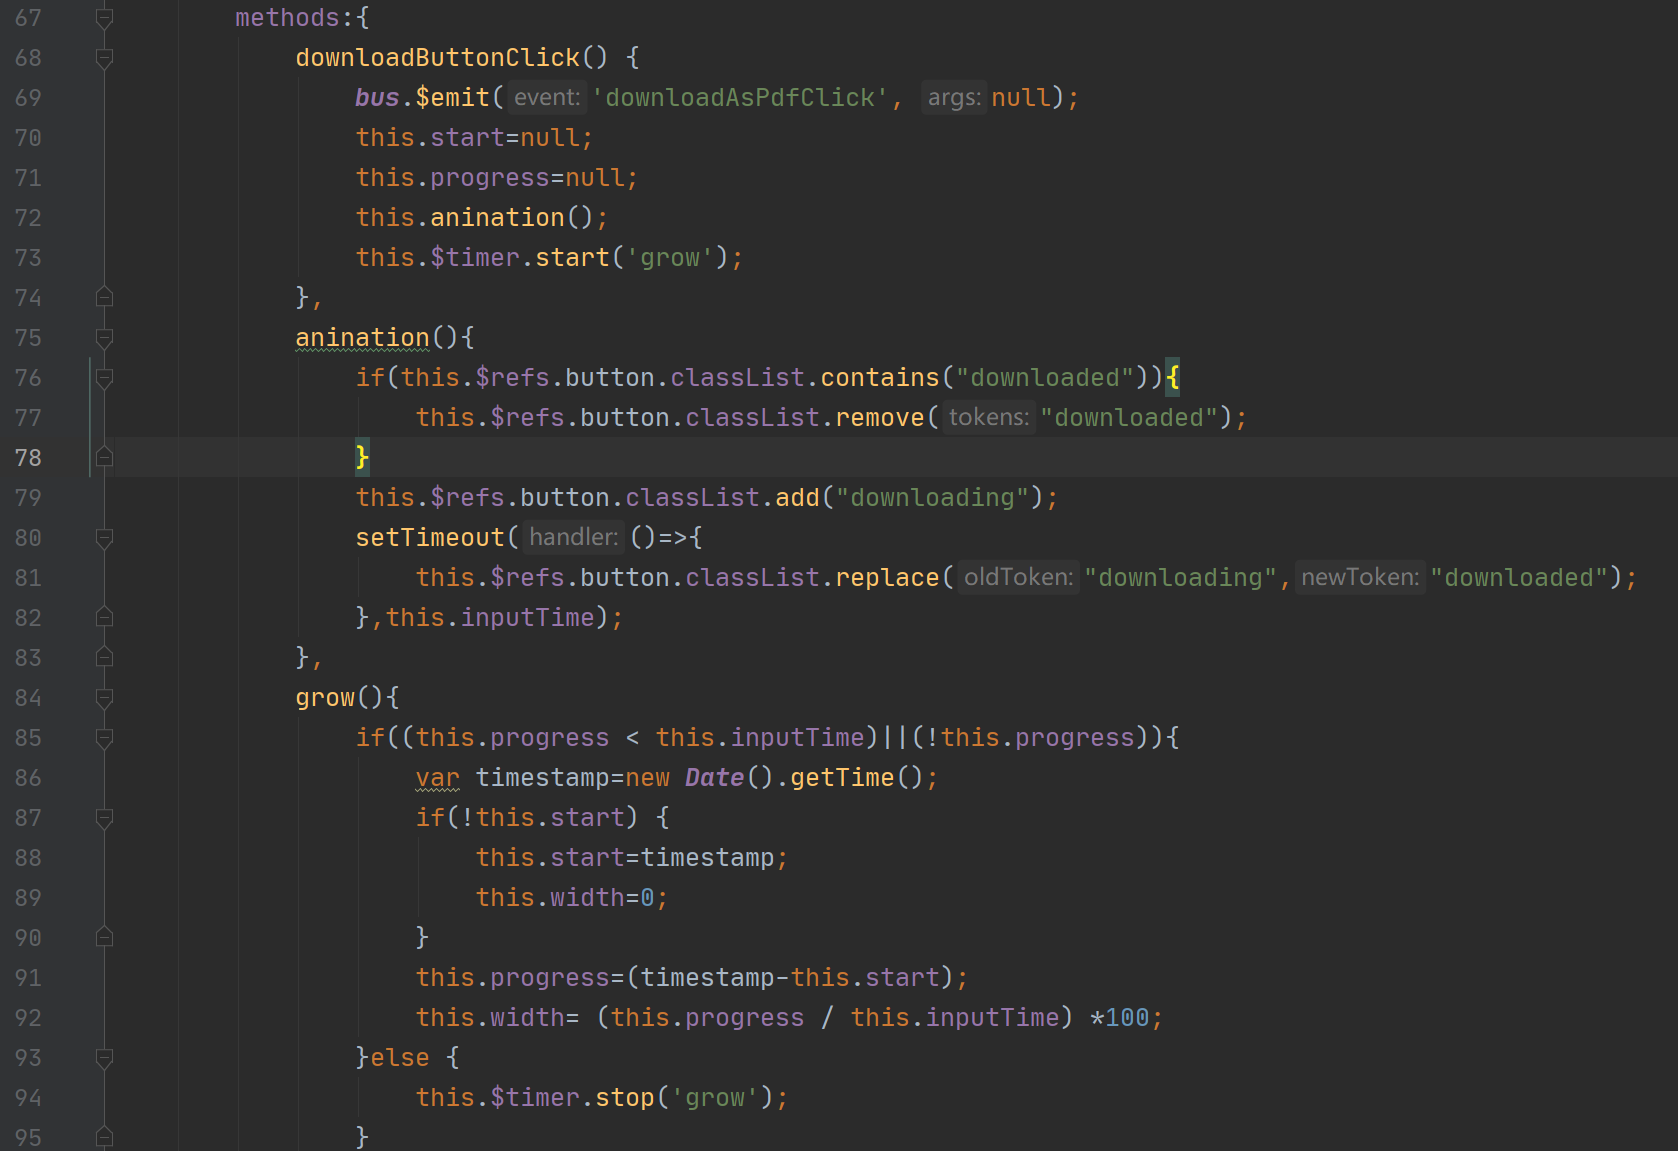
\includegraphics[scale=.4]{figures/downloadButtonJS.png}
		\caption{resume template}
		\label{fig:14}
	\end{figure}
	
	\item Dynamically creating and deleting Vue component instances at run-time.
	 \begin{figure}[H]
		\centering
		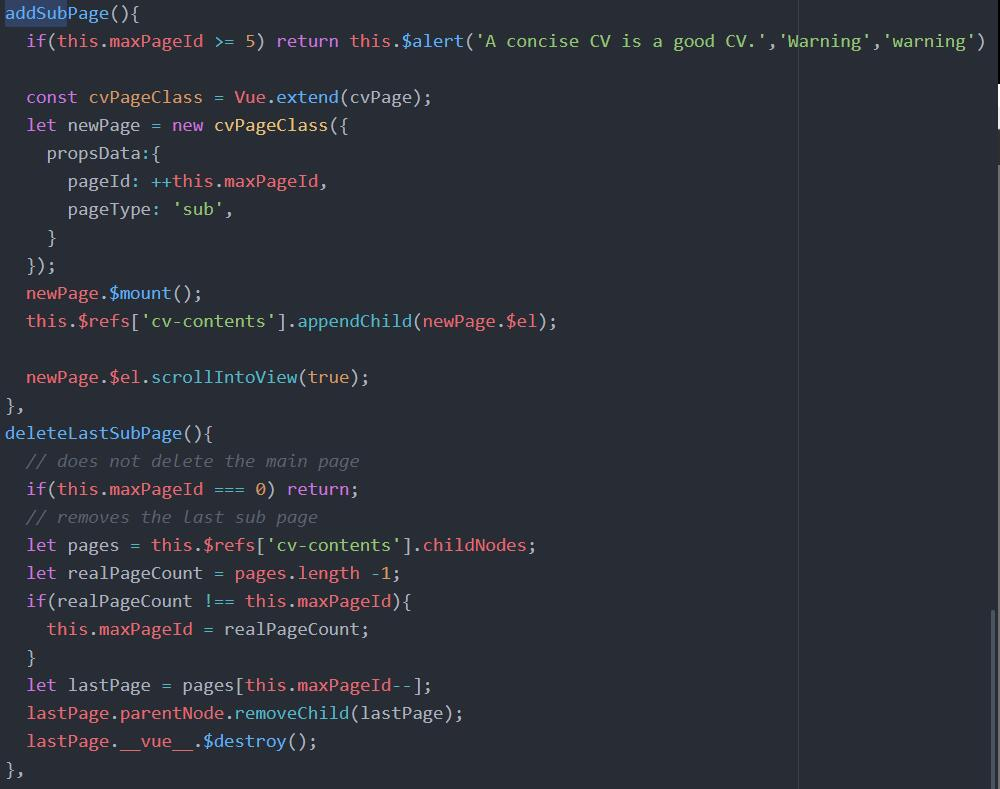
\includegraphics[scale=.5]{figures/js/addSubPage.jpg}
		\caption{dynamic component creation/deletion}

	\end{figure}
	Here is how we implement the add page and delete page at CVMaker page. Each page is an instance of the Vue component "cvMakerPage"
	
	\end{itemize}
	
	\subsubsection{PNG}
	We made all the artworks used in our website by ourselves except the background image, which was free to use and no need to mention the source.
	The licence of the background image could be found here:
	 $https://www.pexels.com/es-es/foto/analisis-analitica-aplicacion-crecimiento-590016/$
	 
	\begin{itemize}
	\item 404 page for front-end router.
	
	We used GMIP for painting. The source file of the 404 page is saved in $src/view/index/img$. We used masks, filters and transparent alaph channels, among other techniques.
	\begin{figure}[H]
		\centering
		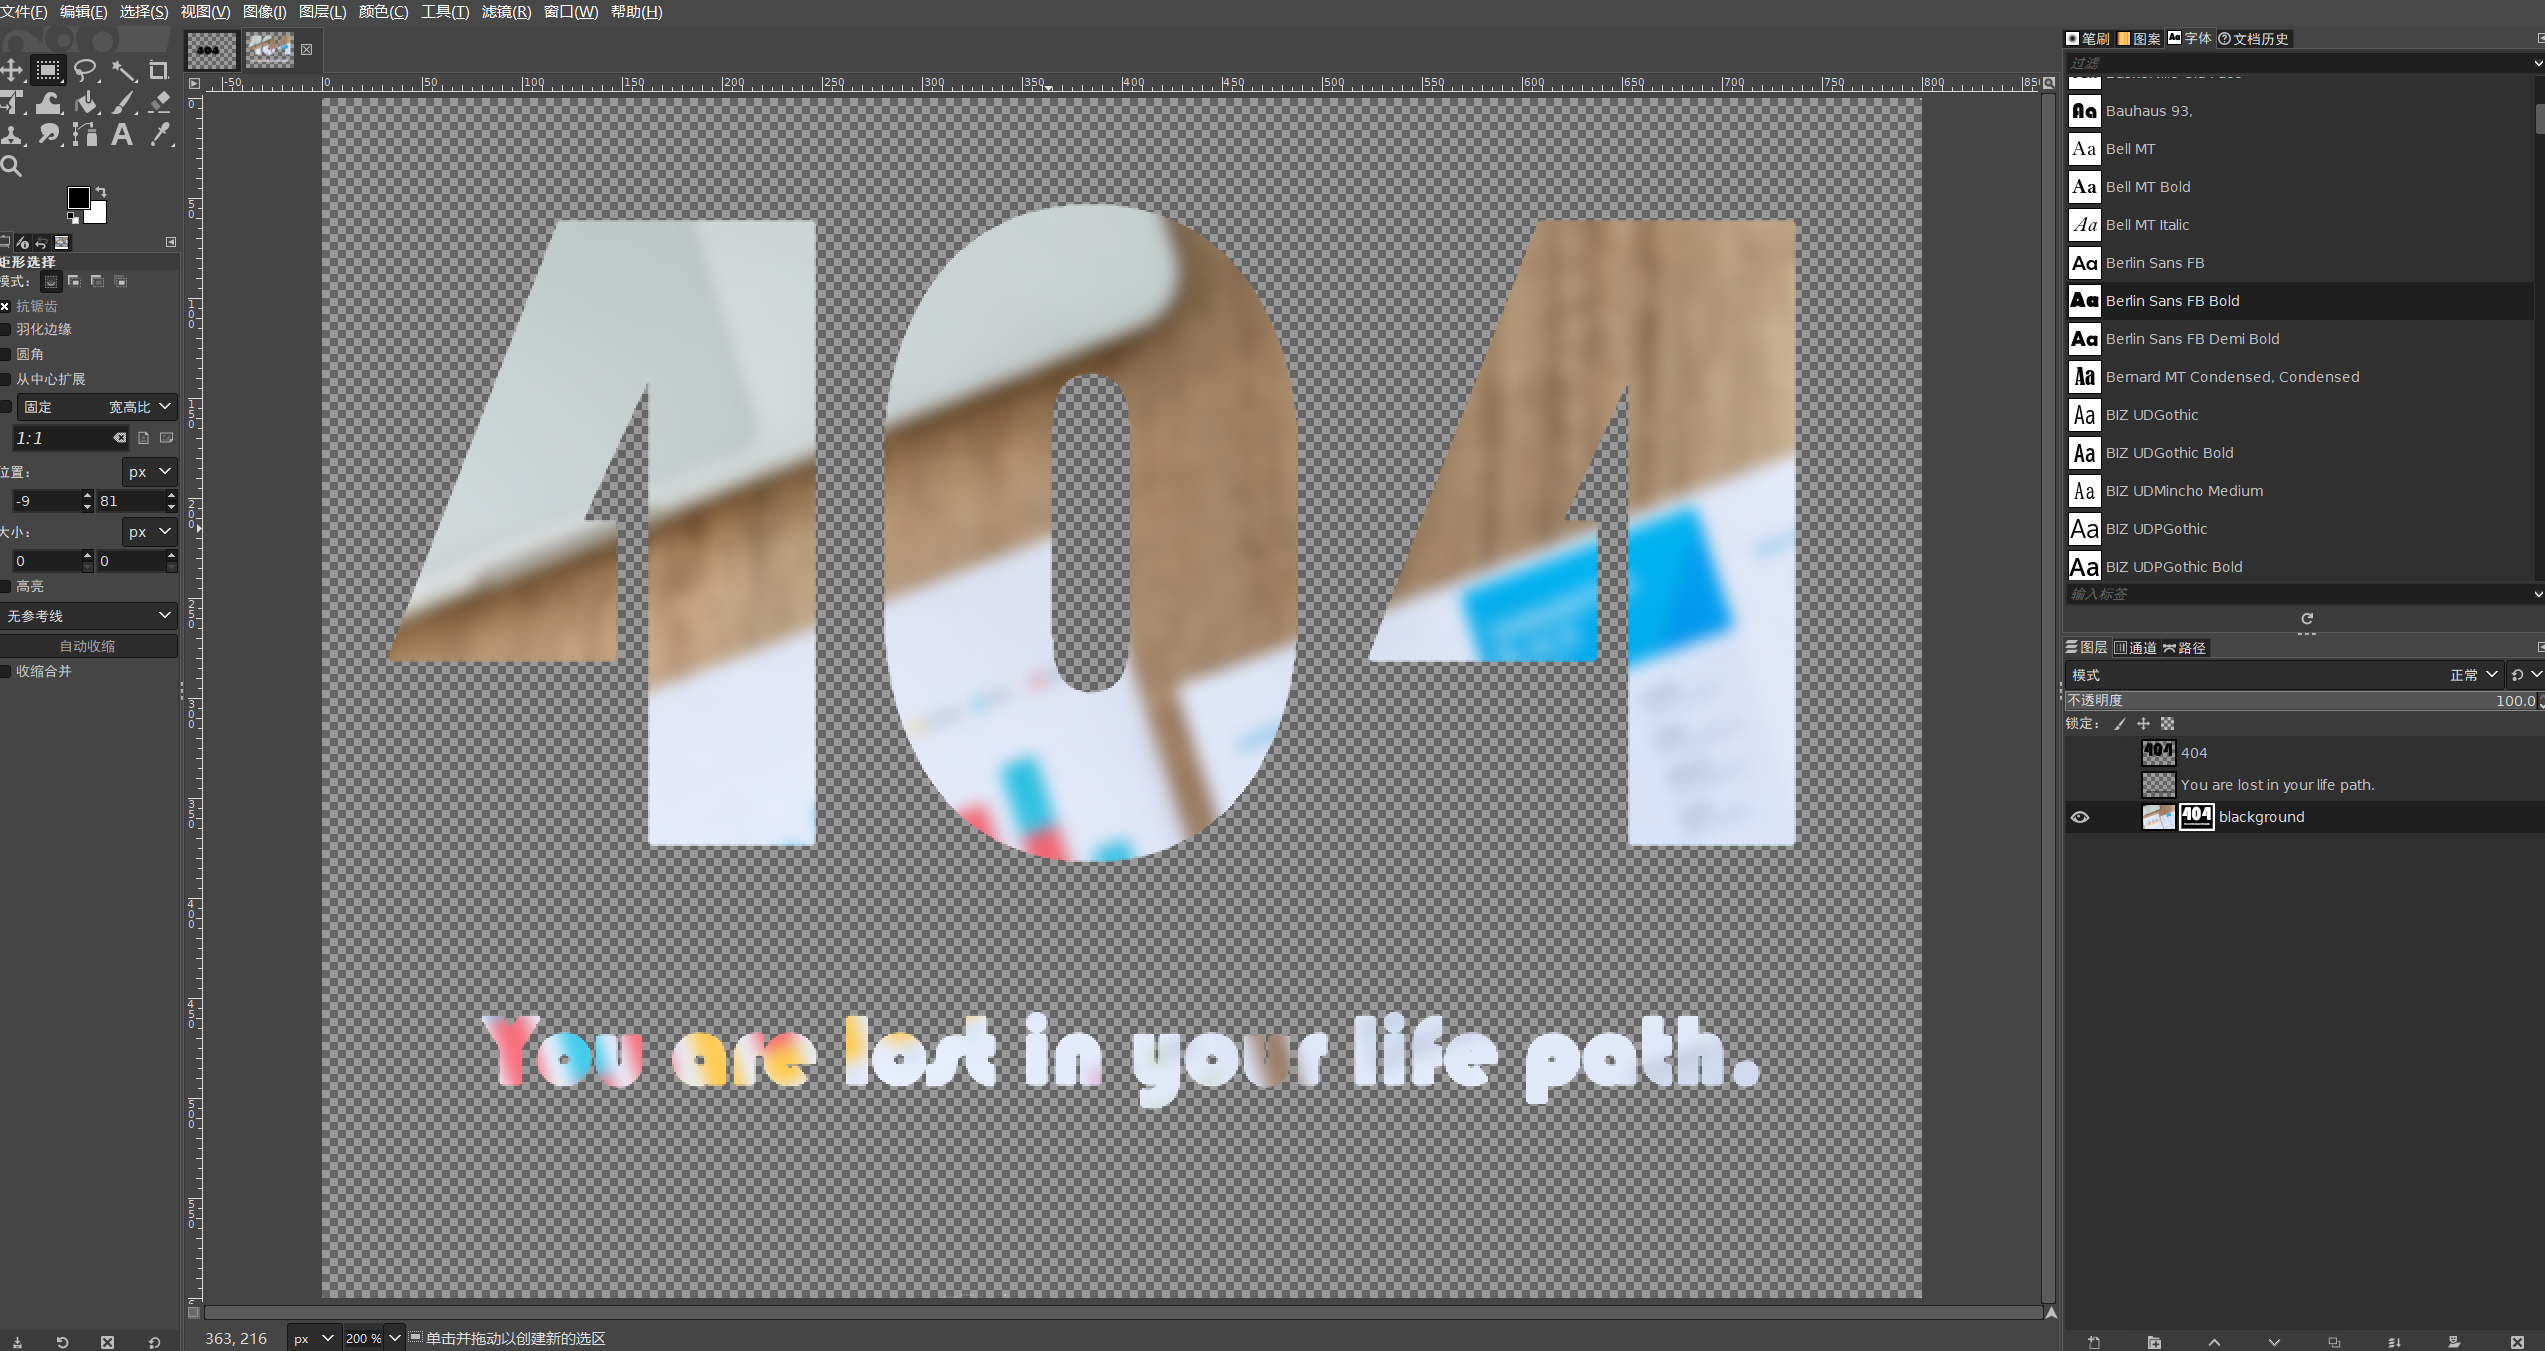
\includegraphics[scale=.3]{figures/404.png}
		\caption{404.png}
		\label{fig:13}
	\end{figure}
	
	check it out:
	\href{https://royalcvmaker.uk/#/Imlost}{Non-existing page}.
	
	\item back-end 404 page.	
	
	Progress:
	\begin{figure}[H]
		\centering
		
\includegraphics[scale=.4]{figures/png/1.jpg}
		\caption{1}

	\end{figure}
	\begin{figure}[H]
		\centering
		
\includegraphics[scale=.4]{figures/png/2.jpg}
		\caption{2}

	\end{figure}
	\begin{figure}[H]
		\centering
		
\includegraphics[scale=.4]{figures/png/3.jpg}
		\caption{3}
	
	\end{figure}
	\begin{figure}[H]
		\centering
		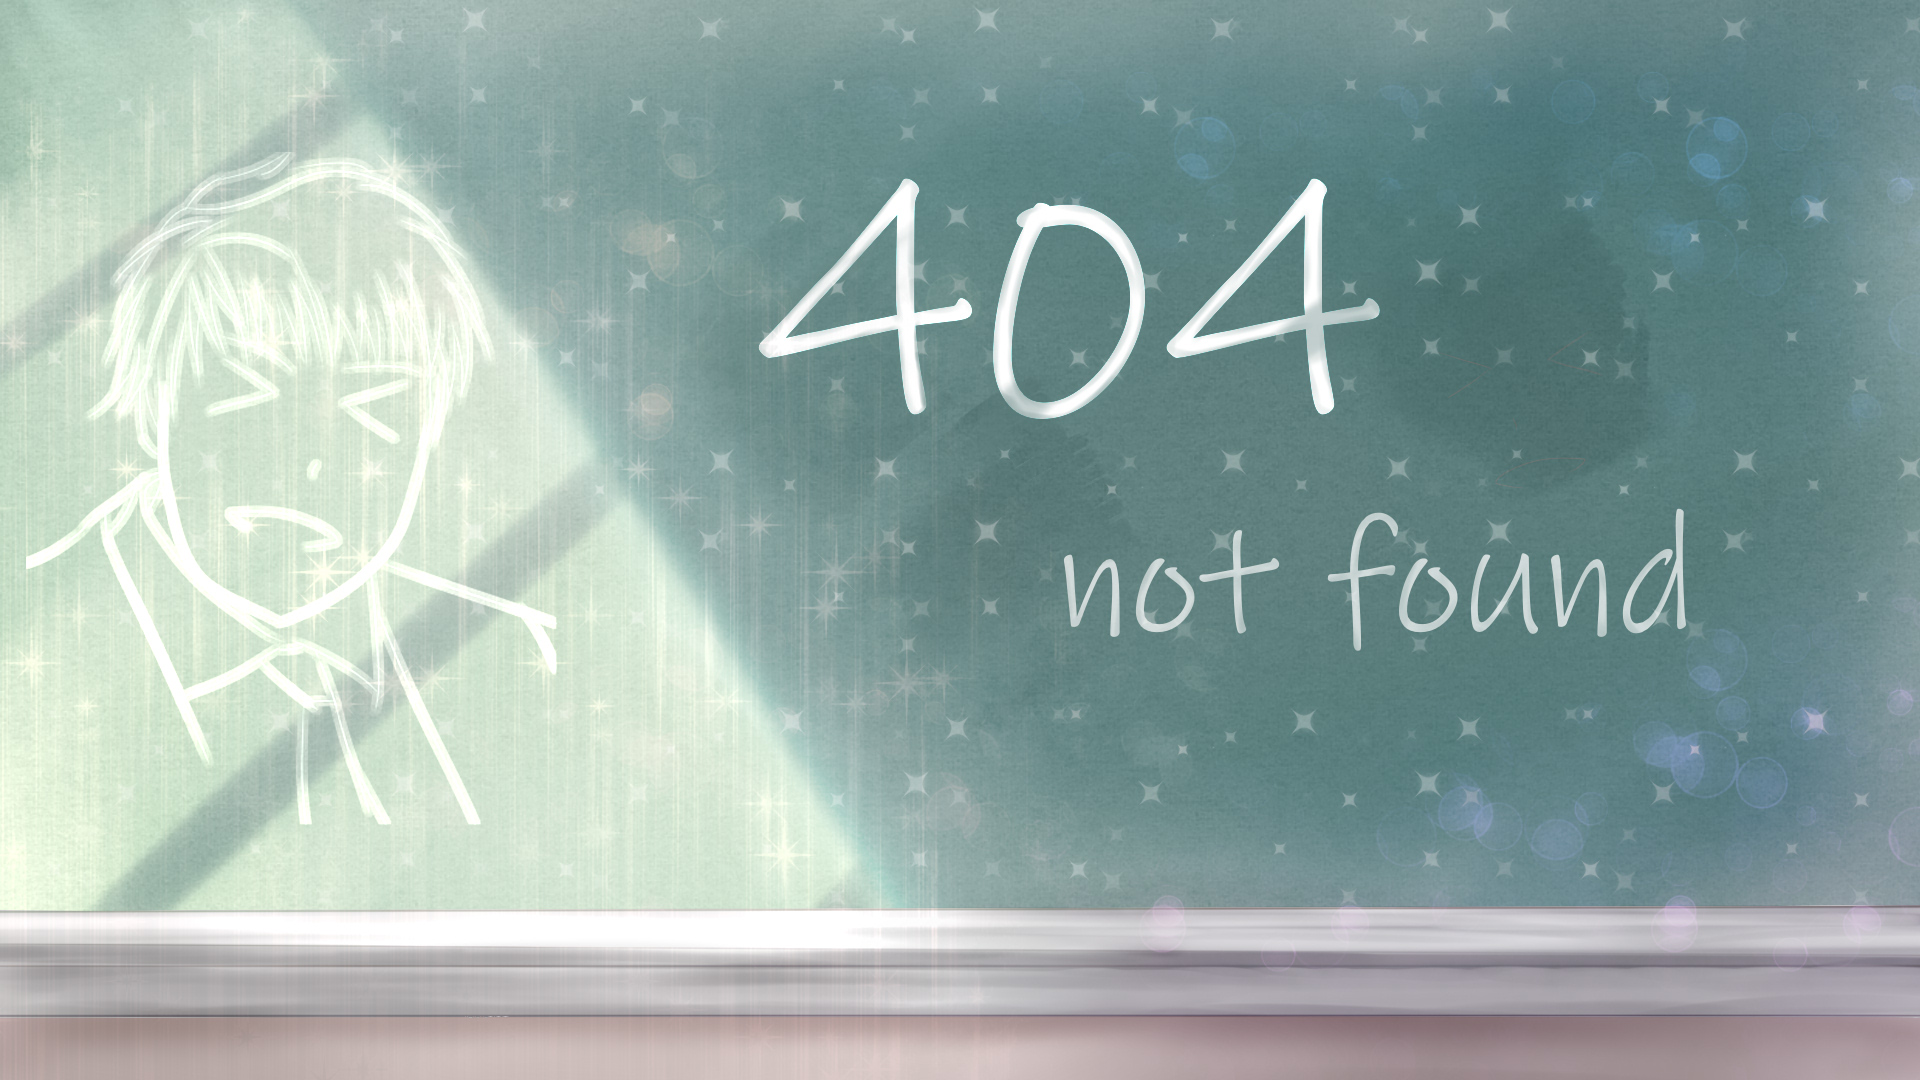
\includegraphics[scale=.4]{figures/png/4.jpg}
		\caption{4}

	\end{figure}
	\begin{figure}[H]
		\centering
		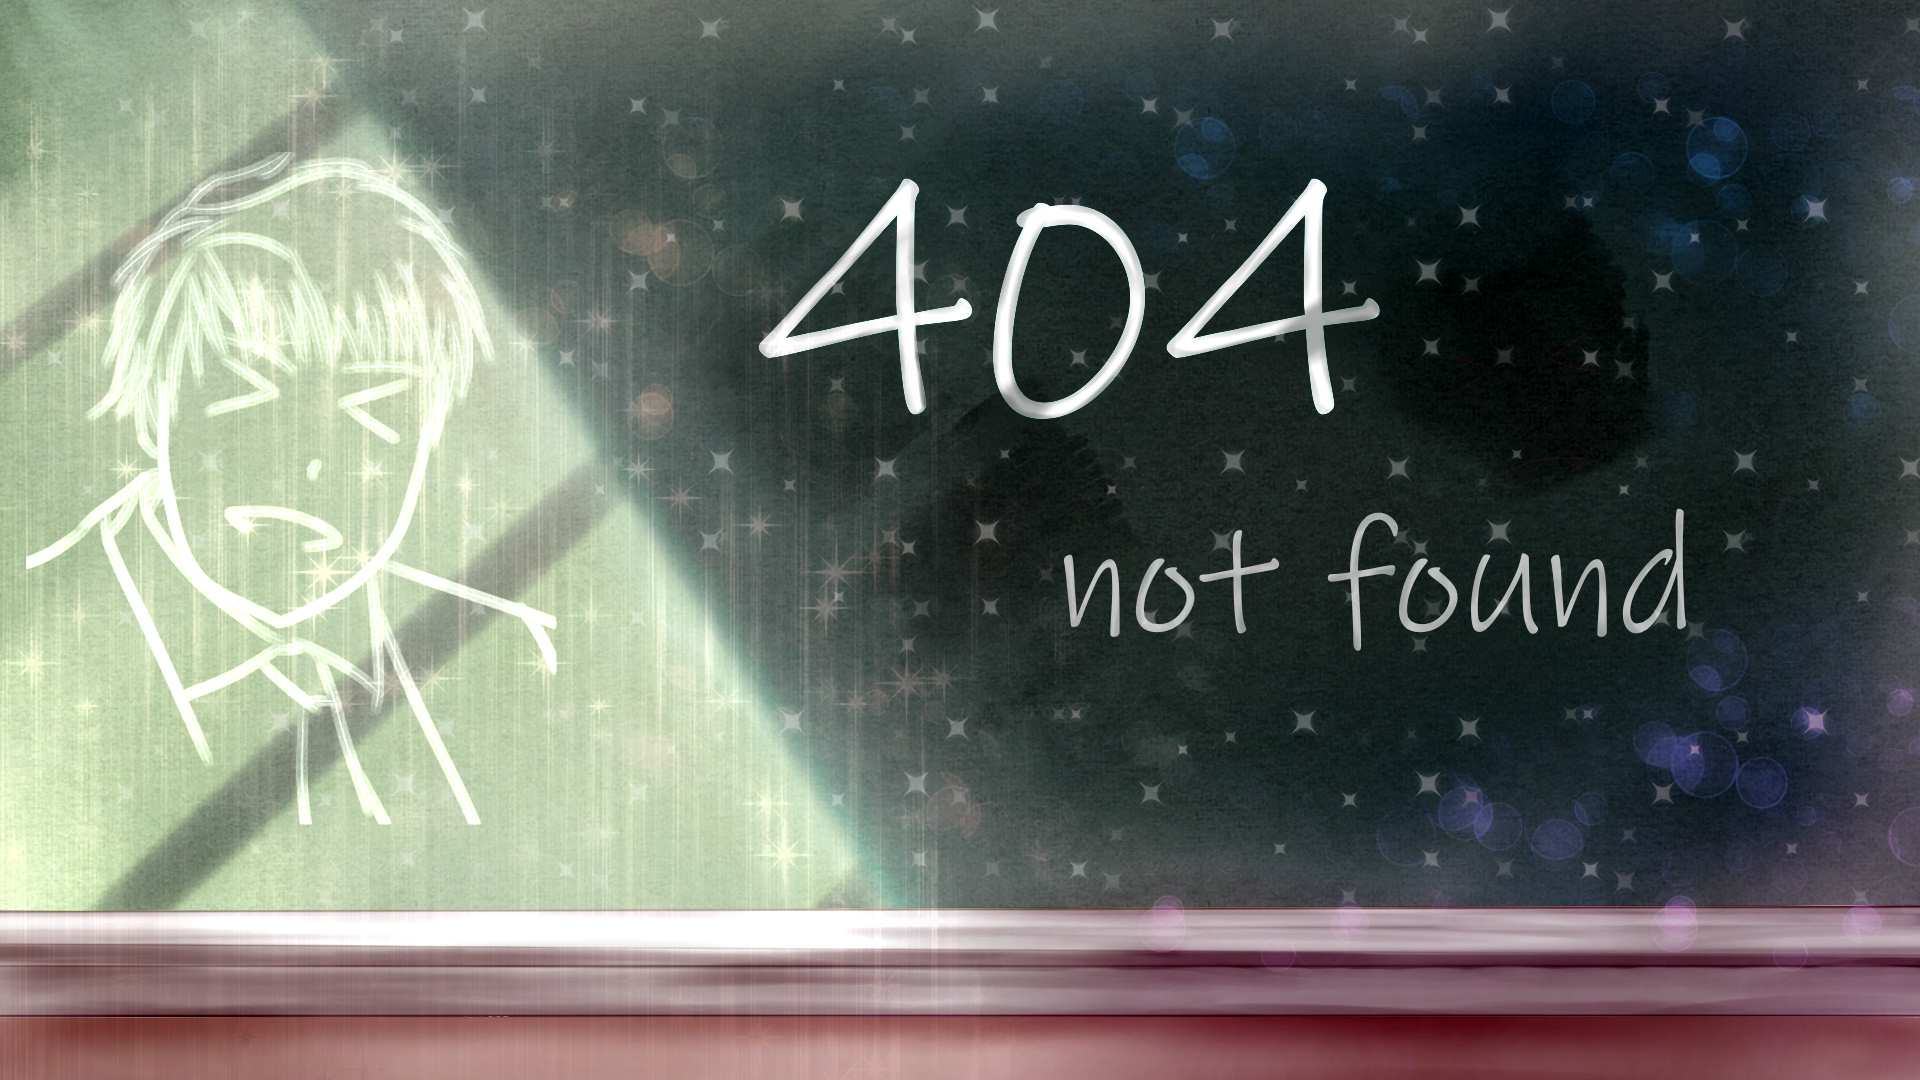
\includegraphics[scale=.4]{figures/png/5.jpg}
		\caption{5}

	\end{figure}
	\begin{figure}[H]
		\centering
		
\includegraphics[scale=.4]{figures/png/6.jpg}
		\caption{6}

	\end{figure}
	

	\begin{figure}[H]
		\centering
		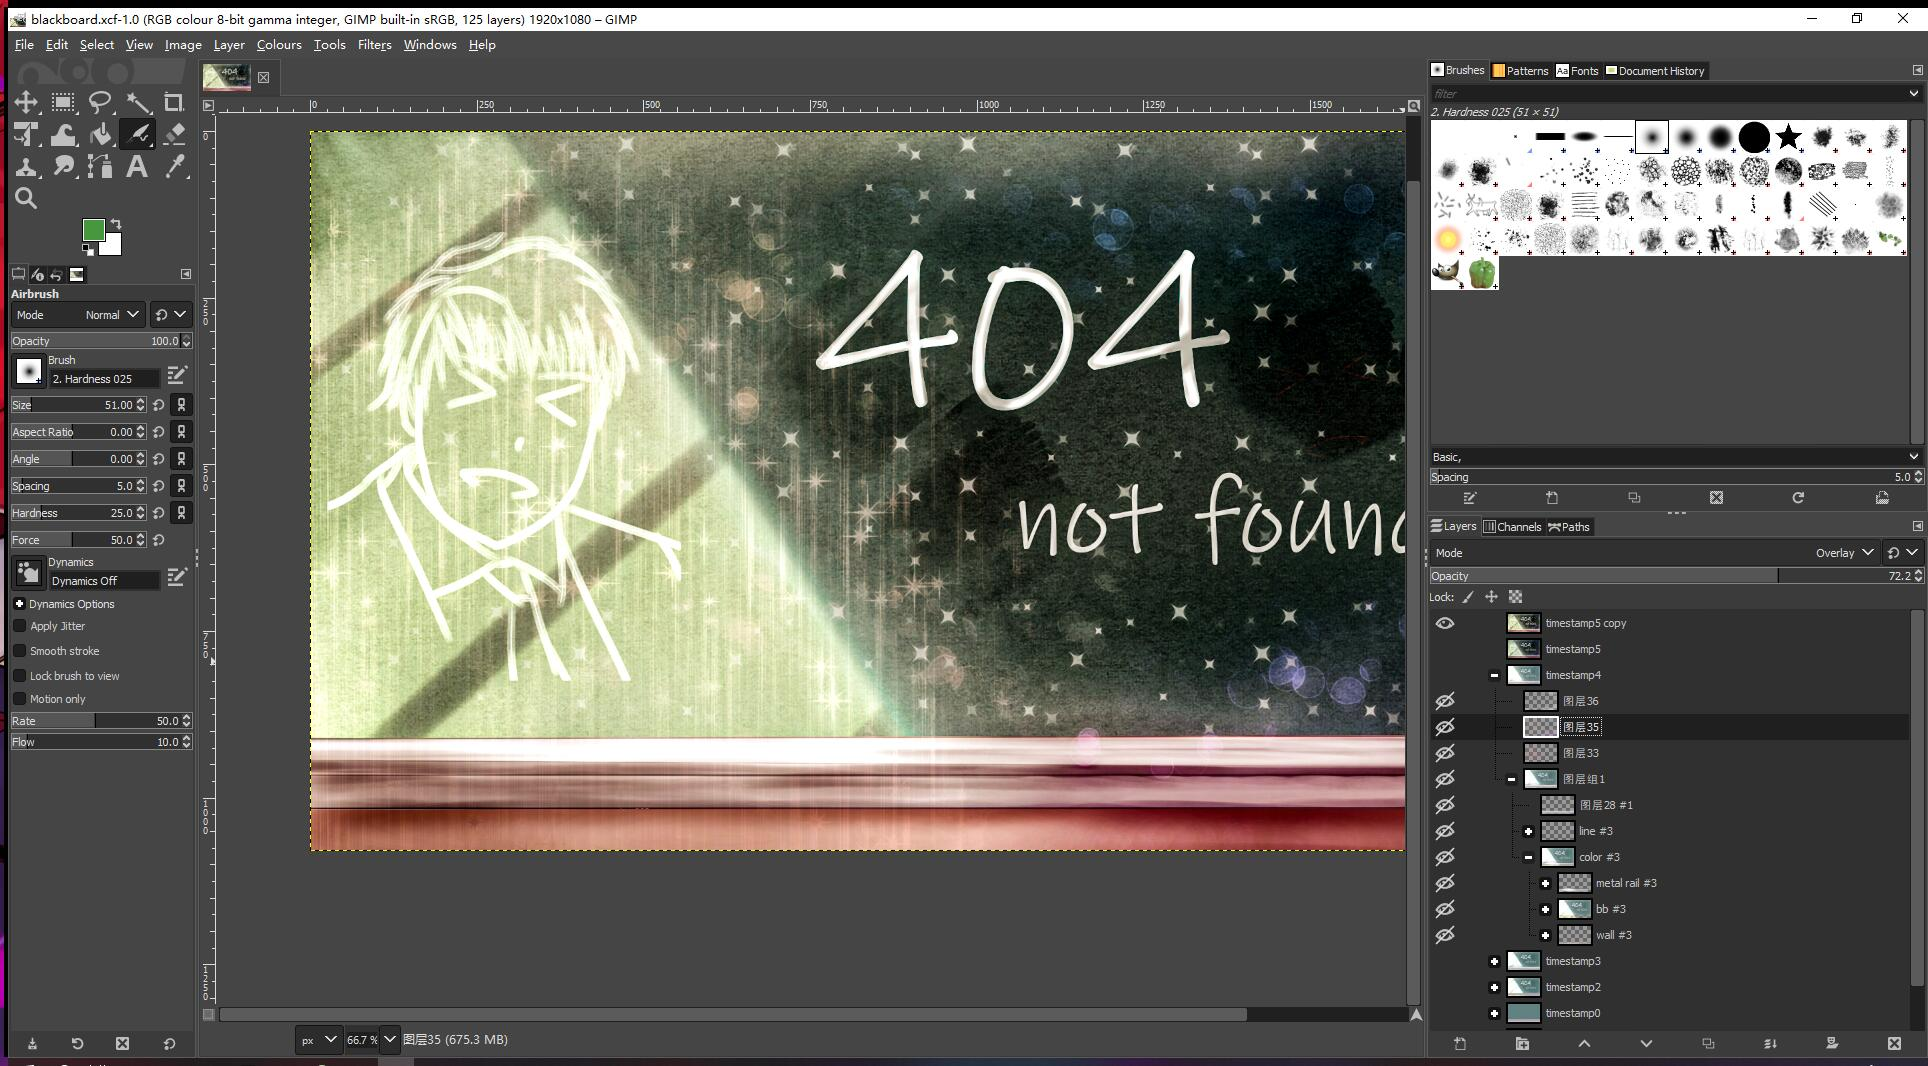
\includegraphics[scale=.3]{figures/png/gimp.jpg}
		\caption{workspace}

	\end{figure}
	Basically, I used paintbrush and airbrush for coloring. "Multiply" and "linear burn" were used as the blending modes for shadow layers, while "addition" was used for highlights. "Overlay" was used for adding opposite or distant colors to some places to make the image appear more vivid, while transparency was adjusted to mitigate effects.
	
	check it out:
	\href{https://royalcvmaker.uk/Imlost}{Non-existing page}.
	
	
	\item Example avatar
	\begin{figure}[H]
		\centering
		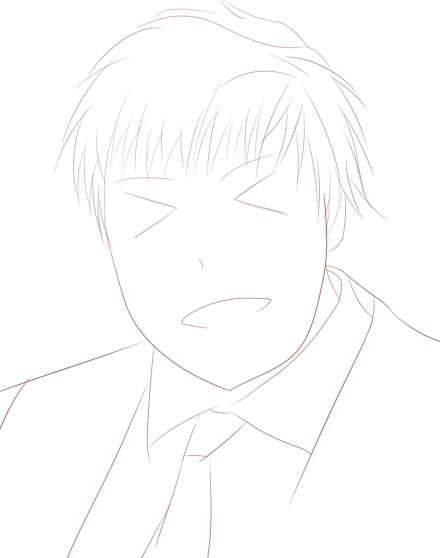
\includegraphics[scale=.5]{figures/png/example_avatar.png}
		\caption{example avatar}
		
	Above artworks pale into insignificance compared to this masterpiece. This is the best picture that I have drawn in my entire life. Detailed facial features, vibrant colors, with the solemn expression as the finishing touch indicating the harsh reality that the concurrent white collar is facing. If this masterpiece is not going to be passed down generation to generation, I don't know what art is all about.

	\end{figure}	
	
	
	\end{itemize}
	
	
	\subsubsection{SVG}
	We have used a variety of ways to construct SVG images to make full use of its advantages. We even created SVG  animation on the home page. We will describe this in detail below.
	\begin{itemize}
		\item Basic SVG images\\
		We used tools like Inkscape to draw simple SVG portraits, and since the team had experience of  adobe Kit, SVG graphics were light work to us. 
		\begin{figure}[H]
			\centering
			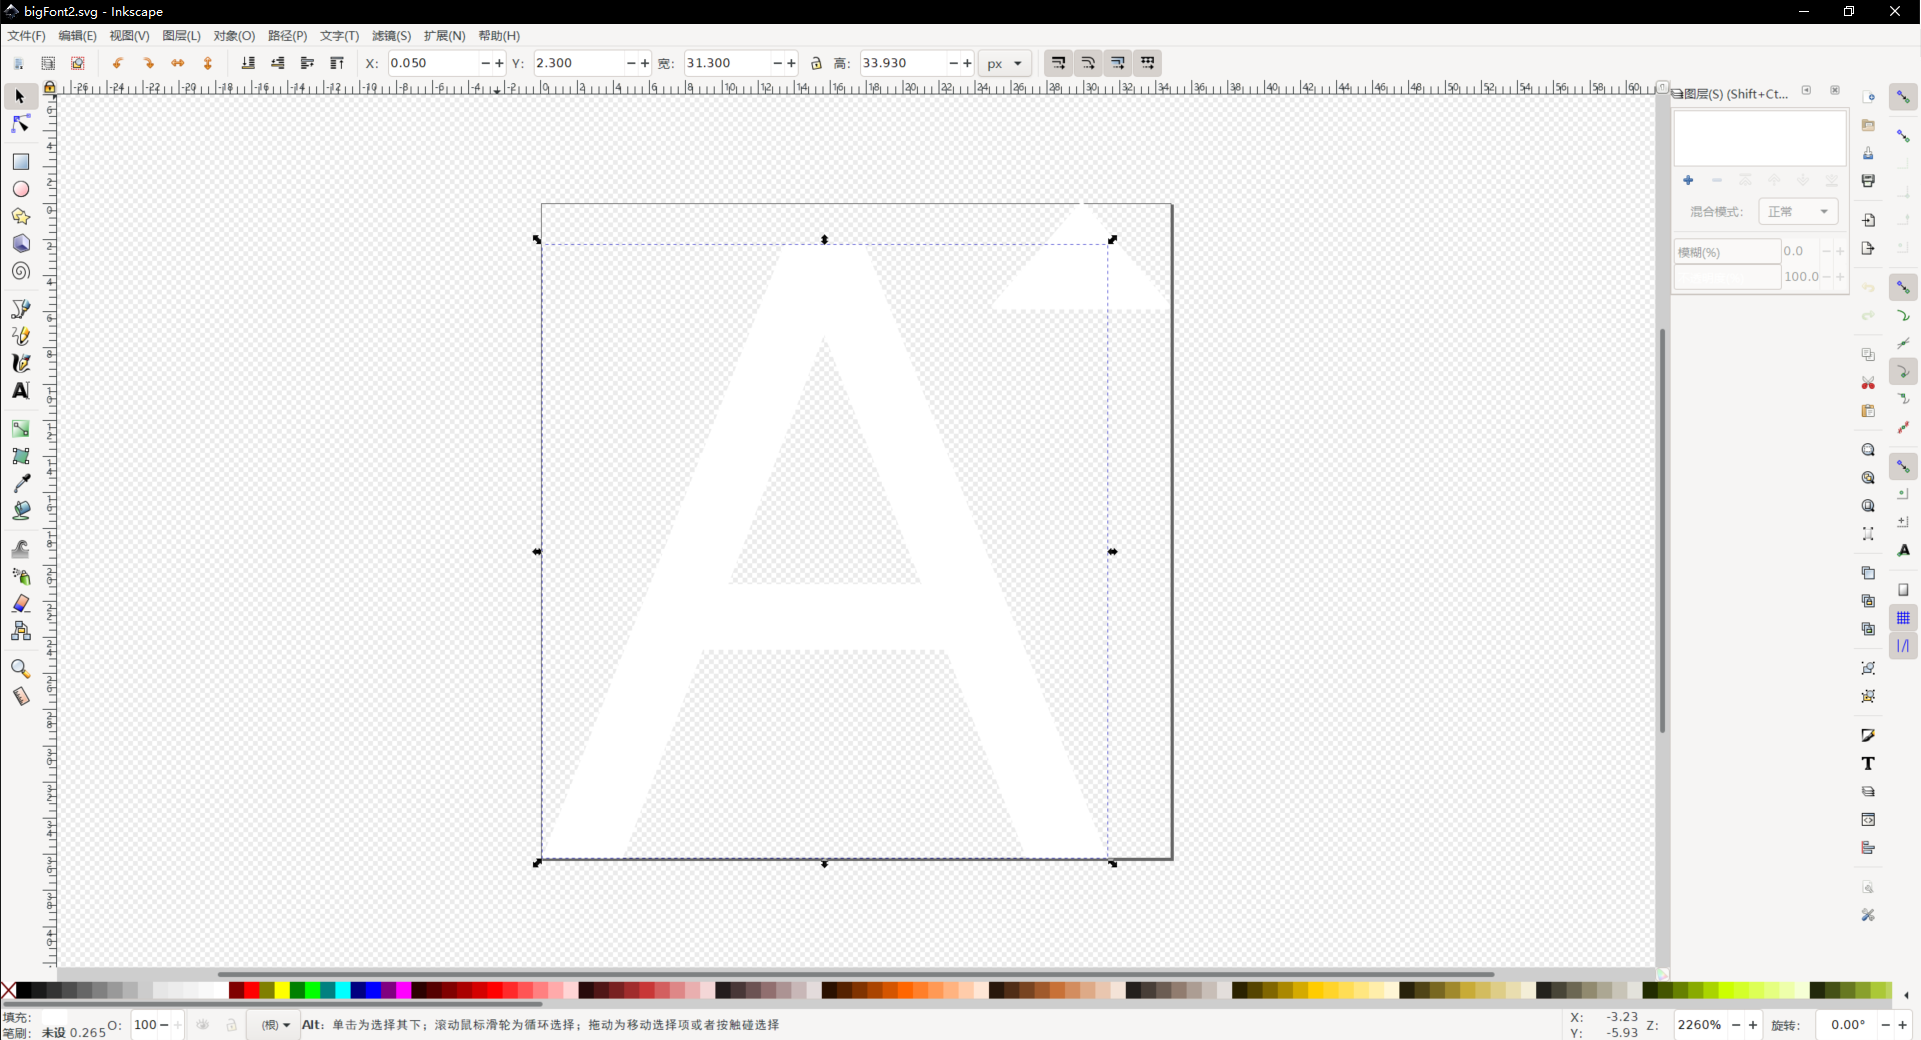
\includegraphics[scale=.3]{figures/svg1.png}
			\caption{Inkscape}
			\label{fig:1}
		\end{figure}
	We used this basic graphical drawing to create 12 buttons, 3 of which are embedded in the page, while the remaining nine are used as Individual components are independent of the elements in the $src/components/button$. We take advantage of the object-oriented component design of the Vue components so that each module is easy to maintain and update later.
	\begin{figure}[H]
		\centering
		
\includegraphics[scale=.3]{figures/buttonBar.png}
		\caption{buttonBar}
		\label{fig:2}
	\end{figure}
	\begin{figure}[H]
	\centering
	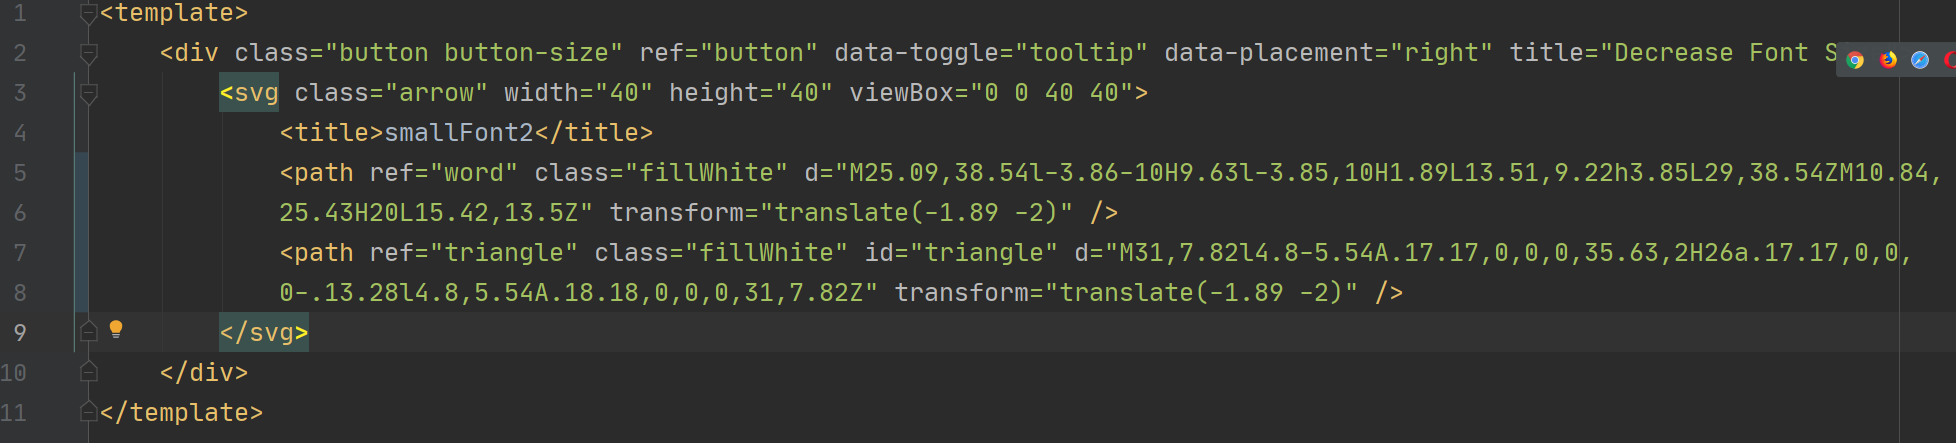
\includegraphics[scale=.3]{figures/smallFontButton.png}
	\caption{smallFontButton}
	\label{fig:3}
\end{figure}
\item SVG-based css animation\\
We were not satisfied with making basic SVG graphics. We created four SVG animations with CSS animation effects. They are the start button on the home page, the continue and new buttons on the user-profile page, and the download button inside CVMaker. The most complex one is the download button, which activates the animation by changing the button's class when clicked. 
\begin{figure}[H]
	\centering
	
\includegraphics[scale=1]{figures/downloadButton.png}
	\caption{downloadButton animation}
	\label{fig:4}
\end{figure}
The download animation is divided into four parts, the first is the flashing of the outer ring, the second is the downward movement of the vertical line in the middle, and the third is the download of The middle arrow pattern becomes a checkmark when finished, and the fourth is the download progress bar at the bottom.
\begin{figure}[H]
	\centering
	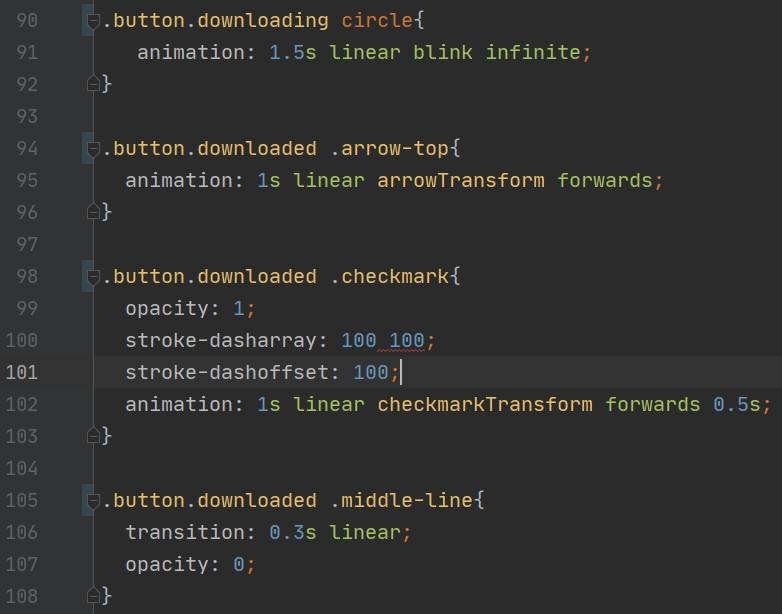
\includegraphics[scale=0.5]{figures/cssAnimation.png}
	\caption{downloadButton animation}
	\label{fig:5}
\end{figure}
\item svg animation based on vue-lottie\\
Of course, doing this will not satisfy our ambition to try the coolest animations. So we introduced the vue-lottie open-source package, which is based on the \href{https://github.com/airbnb/lottie-web}{lottie}. Vue-lottie project vue architecture lottie can be interpreted as an SVG animation interpreter, and he supports the use of SVG in adobe After Effects exports complex animations to a JSON file and then self-rendering through the front-end of the web page to get cool effects.

We've made a dynamic animation on the home page to highlight our theme, which we're sure you've seen.We save the exported animation JSON file that we send to AE in the $src/view/index/assets/animation$ folder.
\begin{figure}[H]
	\centering
	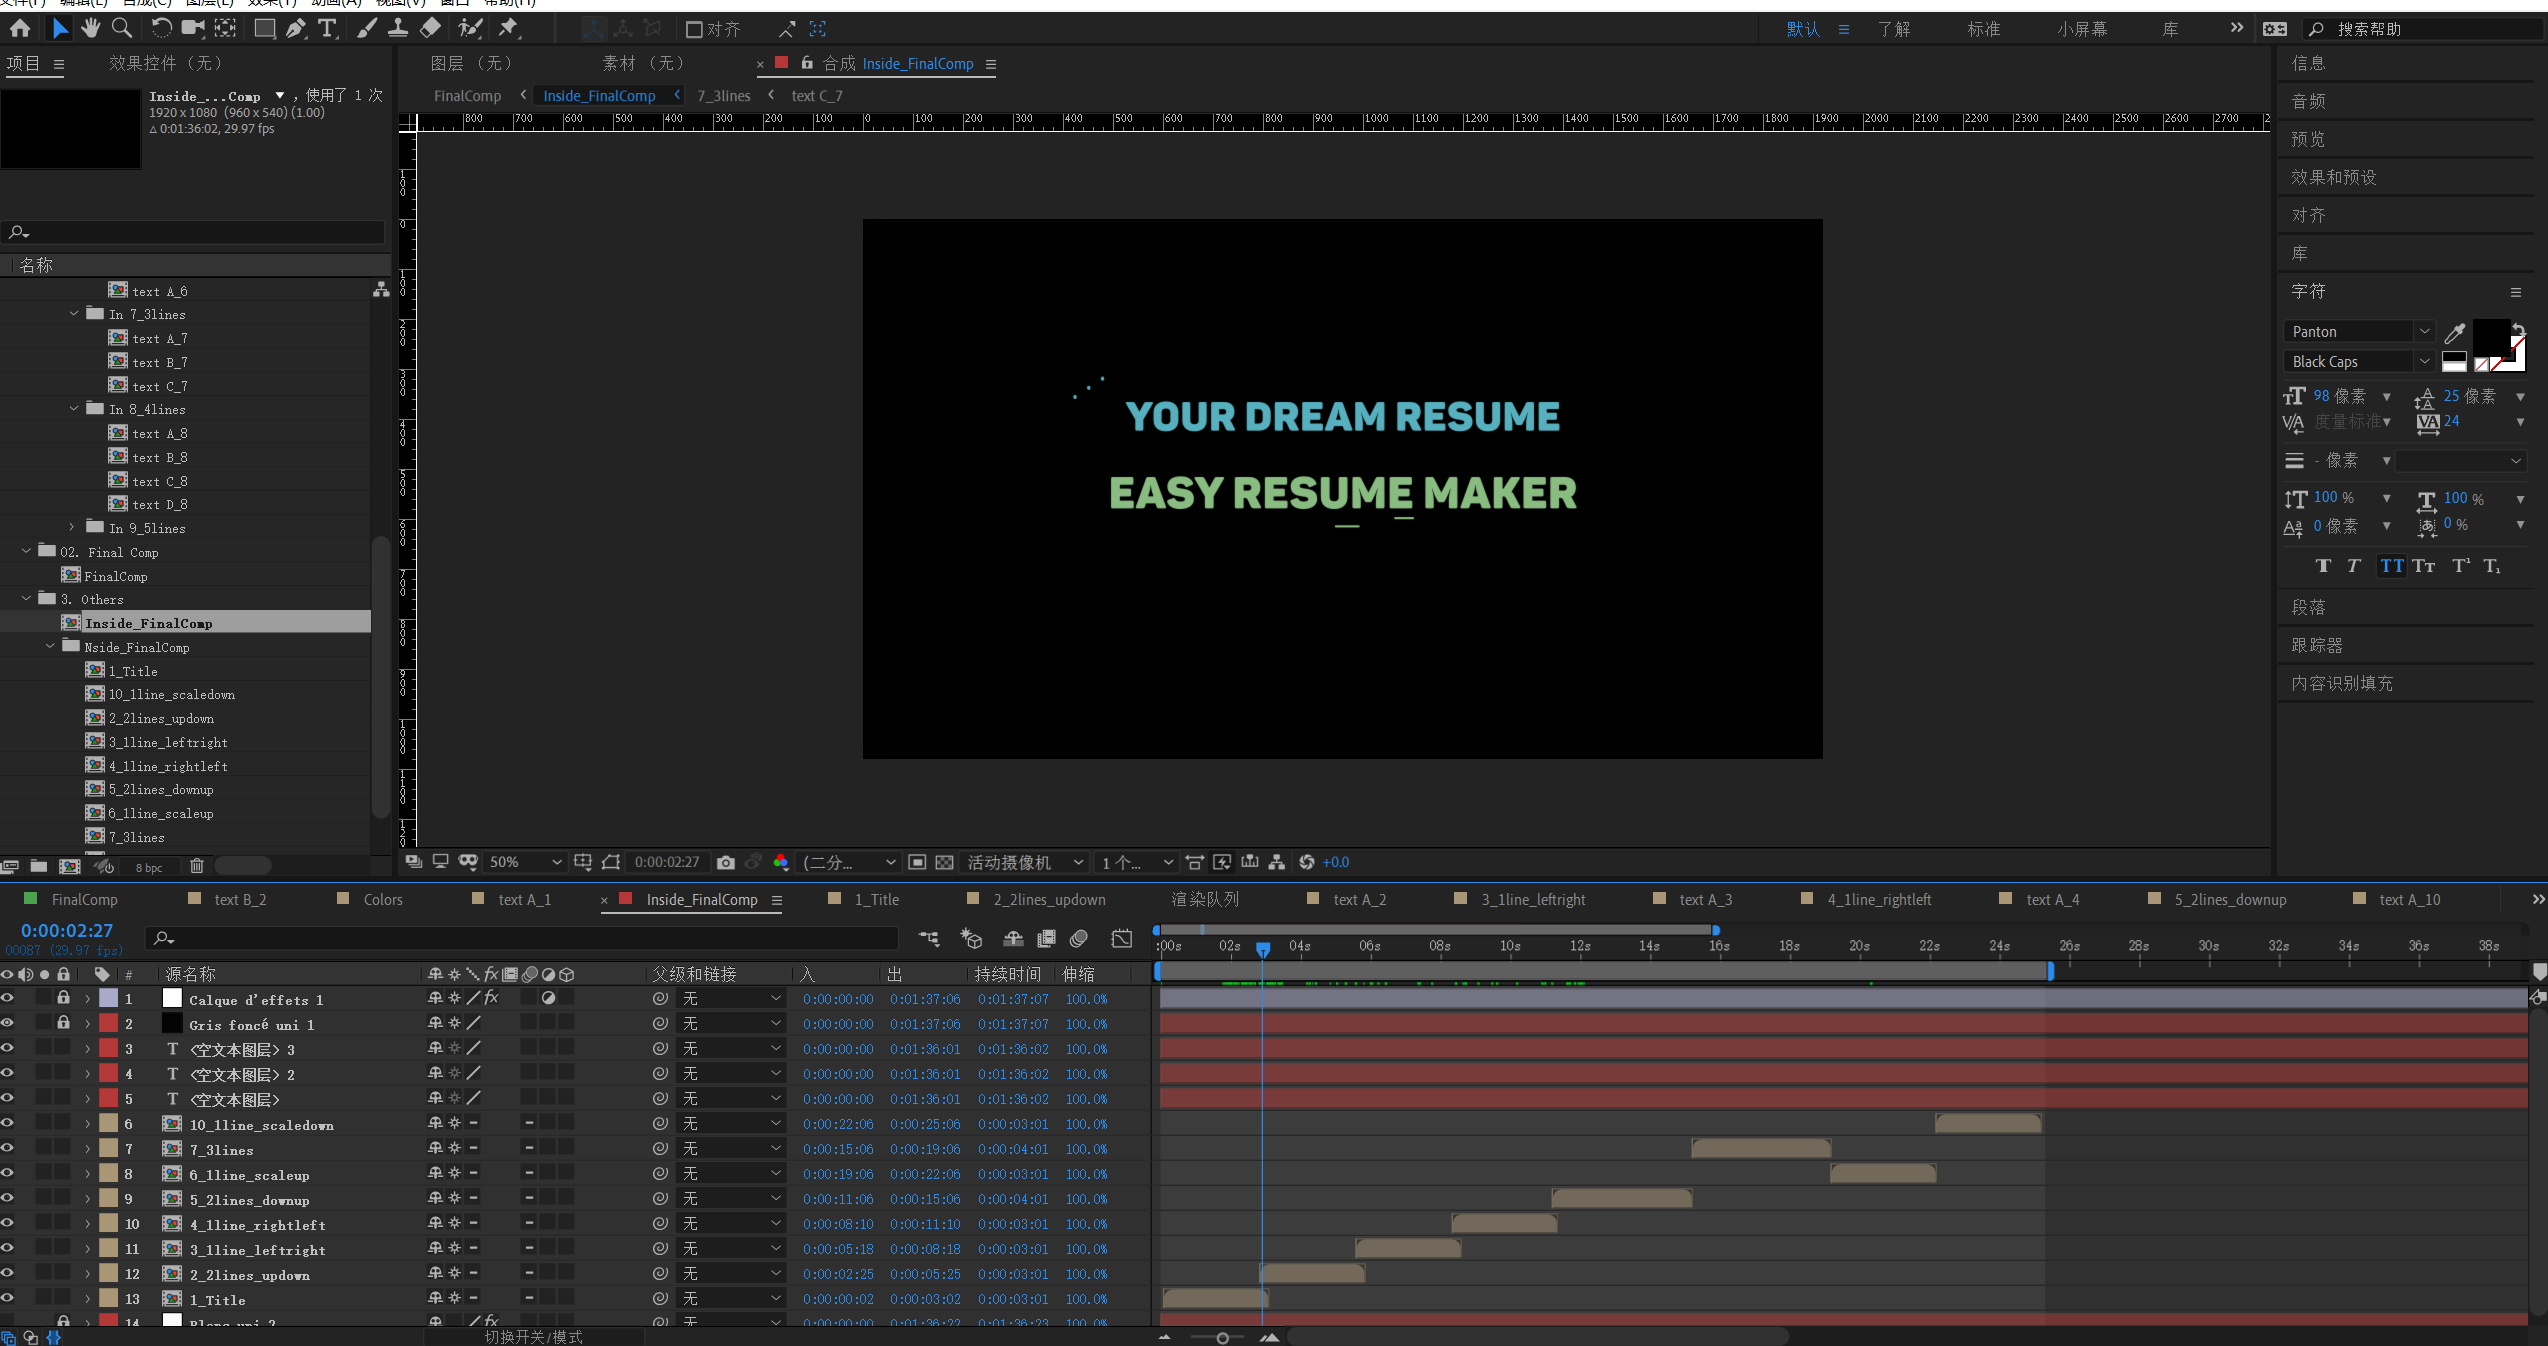
\includegraphics[scale=0.2]{figures/ae.png}
	\caption{After Effect}
	\label{fig:6}
\end{figure}
Since this lottie tool is so new, we think we have made it pretty far ahead of the curve in terms of SVG usage.

	\end{itemize}
	\subsection{Server Side}
	\subsubsection{Server}
	
	\begin{itemize}
	

	\item Port numbers
	
	Port numbers are read from process.env if they exist. Otherwise, 80 and 443 were used for http and https, respectively. 
	
	\item Https and http redirect
	
	The server runs on https mode by default. There is another http server that redirects the users to https if they attempt to connect via http.
	
	For localhost, a self-signed certificate was used for development and demonstration of concept, although some browsers will complain about that.
	For our cloud server, we successfully applied one from ZeroSSL RS Domain Secure Site CA. This certificate and its corresponding key are not included in this repository for security concerns, but their presence could be verified by visiting our website at https://royalcvmaker.uk
	
	\item Cloud hosting
	
	We are hosting this website at https://royalcvmaker.uk
	
	\item JSON web token (JWT) and cookies
	
	JWTs was used both to identify users and to provide some level of security since they are encrypted.
	When a user successfully logs in, a JWT containing their userId will be issued for them. After receiving the JWT, it will be stored in the cookies, so subsequent requests by the user will contain the JWT. All sensitive operations (e.g. get avatar, load CV contents) will require verification of the JWT. In this way, the privacy of the users is protected.
	
	($/routes/verifyJwt.js$)

	\item Hashed password
	
	Users' passwords are not stored in the database directly. Instead, their hashes are stored. Whenever a user request to login, their password is passed to the same hash function and then be compared with that stored in the database, which provides some level of security. We used the node module "bcrypt" to accomplish this task.
	
	($/routes/auth.js$)
	
	\item Validation of request
	
	Some important or complex requests are validated before being processed in order to give users some information (when register/log in) or just check the validity of the request (when save progress). 
	
	($/util/validation.js$)
	
	\item Wrap some callback-styled library methods in Promises so they fit better in this project, whose main style is async-await.
	
	($/util/async_fs.js$)
	
	($/util/dbManager.js$)
	
	\item Most importantly, the server works fine.
	
		\end{itemize}
	\subsubsection{Database}
	\begin{itemize}
	\item All access to the database is done via our module "dbManager", although some query strings may reside somewhere else for simplicity.
	
	($/util/dbManager.js$)
	
	\item Callback style methods that we needed were wrapped in Promises so that they could be used with async-await syle.
	
	($/util/dbManager.js$)
	
	\item Database schemas were placed in a separate file for easier management. 
	
	($/util/dbSchemas.js$)
	
	\item Auto setting up the database when the server starts and if the database folder is not found.
	
	($/util/serverInit.js$)
	
	($/util/resetDb.js$)
	
	\item Auto updating CV template info into the database when the server starts.
	
	($/util/dbInsertTemplates.js$)
	
	\item Update/insert/extract data without problem. The database works fine.
	
	Here is an example update/insert usage of saving users' CV data into the database:
	\begin{figure}[H]
	\centering
	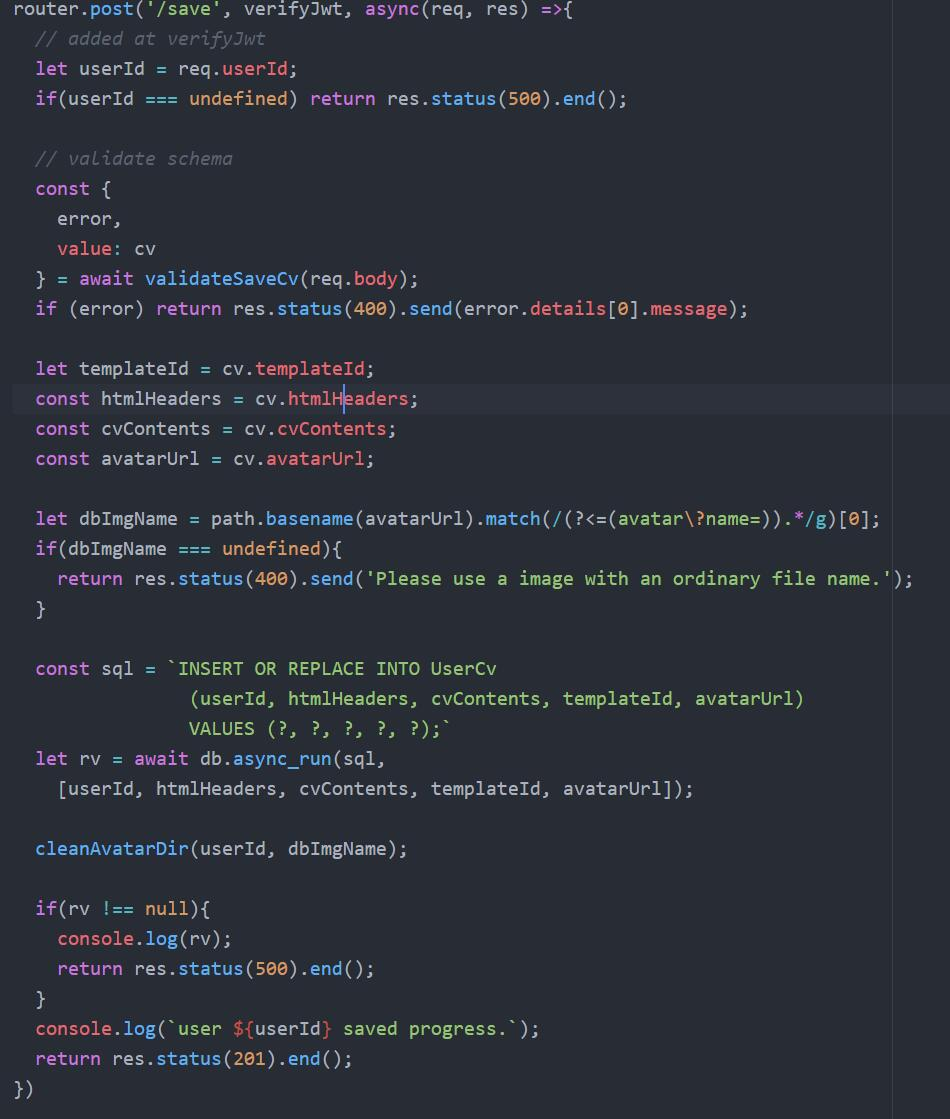
\includegraphics[scale=0.5]{figures/db/save.jpg}
	\caption{save}
\end{figure}

	And this is an example extract usage of retrieving user CV data from the database:
	
		\begin{figure}[H]
	\centering
	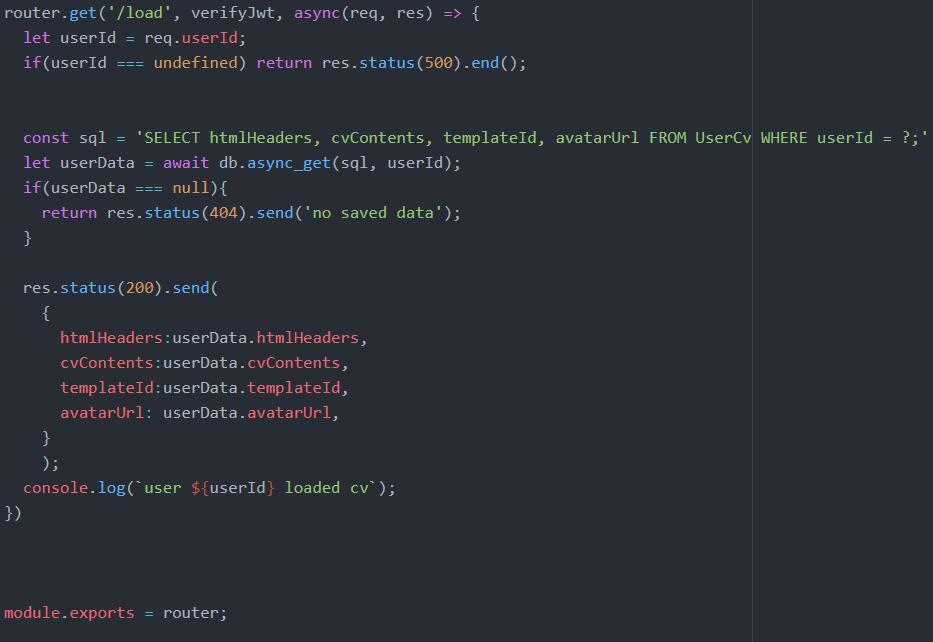
\includegraphics[scale=0.5]{figures/db/load.jpg}
	\caption{load}
\end{figure}
	
	\item Simple command line database management system for debugging which reads sql commands from the command line and query the database with the command and then prints the result to the console:
	
			\begin{figure}[H]
	\centering
	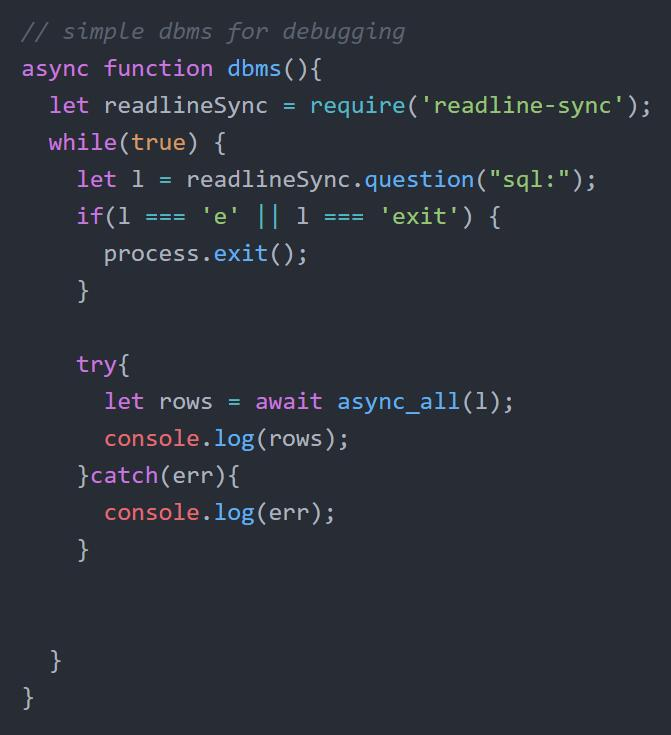
\includegraphics[scale=0.5]{figures/db/dbms.jpg}
	\caption{load}
\end{figure}
	
	
	\end{itemize}
	
	
	\subsubsection{Dynamic pages}
	
	\begin{itemize}
	\item In select template page, templates' information is retrieved from the database when the component reached the life-cycle hook of "created":
	
				\begin{figure}[H]
	\centering
	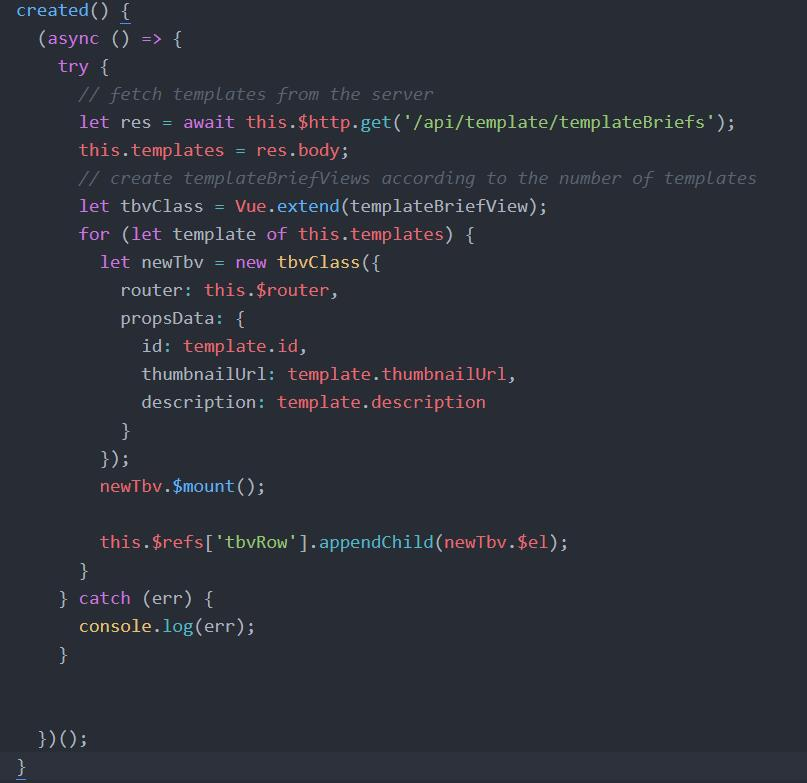
\includegraphics[scale=0.5]{figures/dp/selectTemplate.jpg}
	\caption{select template}
\end{figure}
	
	One instance of the component "templateBriefView" will then be created for each template received. Those instances will then be appended to the right position of the DOM.
	
	As you can see, this dynamic delivery takes advantages of many Vue features. 
	
	($/src/components/selectTemplate.vue$)	
	
	\item The style of CV pages is dynamically loaded.
				\begin{figure}[H]
	\centering
	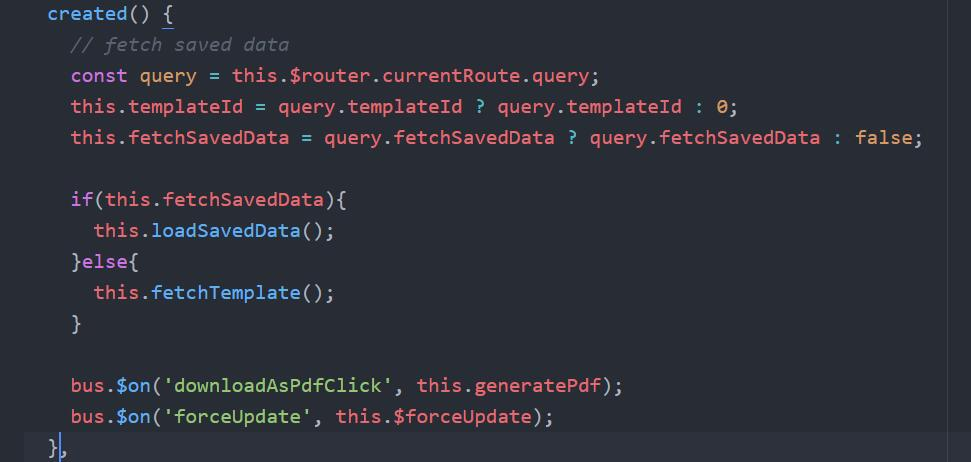
\includegraphics[scale=0.5]{figures/dp/cvMakerCreated.jpg}
	\caption{get template}
\end{figure}	
	
	When the CVMaker component is created, it needs to fetch the CSS for the CV pages from our server, either by loading the user's saved data or by creating a new stylesheet link depending on the query passed by the previous page. 
	
	\begin{figure}[H]
	\centering
	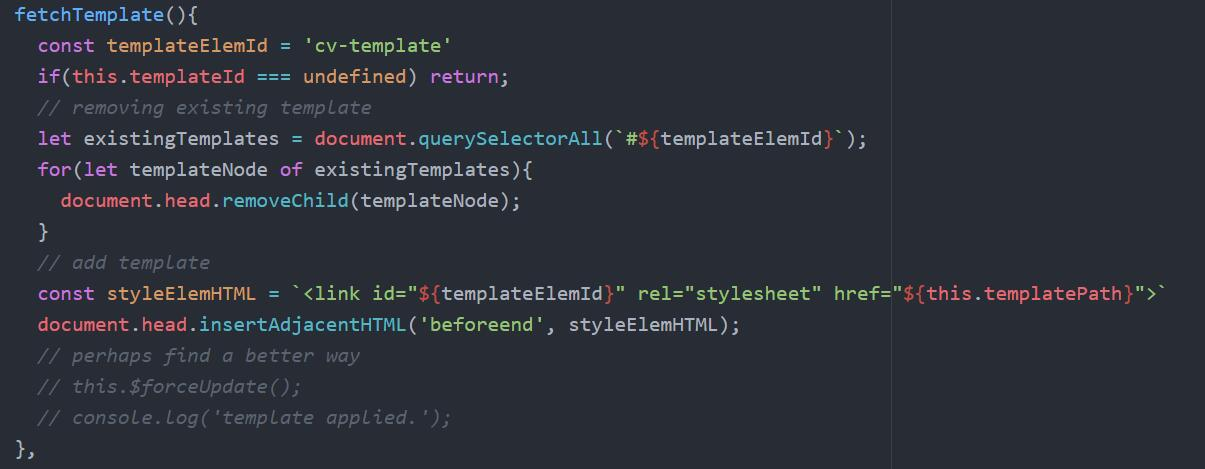
\includegraphics[scale=0.5]{figures/dp/fetchTemplate.jpg}
	\caption{fetch template}
\end{figure}	
	
	As for fetching template, existing template is replaced with the new one by deleting previous "link" tag and inserting new link so the server will responds with the new template.
	
		($/src/components/cvMaker.vue$)	
	
	\item When a user loads their saved progress, what is displayed on their screen will be replaced with what the server responds.
	
	The method that is responsible for this functionality is quite long, so please refer to the source code "loadSavedData" at
	($/src/components/cvMaker.vue$).
	
	Why did we wrote this seemingly complex, typical newbie programmers' not refactored method? And you will find that the "save" method is much shorter than the "load" one. Was it really necessary?
	
	Well, yes. For loading, the "head" tag of the current page is replaced with what is in the server's response directly, and there is no problem with that. However, in the "body" section, we need to be careful with those elements with event listeners. What we did was actually ignoring all elements with event listeners (such as the image uploader).
	
	What would otherwise be an alternative would have been replacing just text instead of html, which would have been a better choice but requiring more labour since the number of elements currently on the page is very likely not the same as that in the saved data, and therefore more logics would have been needed to implement that functionality.
	
	And I have to admit that there is a problem with the existing implementation because the Vue inserts a custom attribute "data-?" as identifier for scoped CSS code and those elements that it affects. The problem is that this attribute is likely to differ each time we compile the frontend, which means if a user saved their data before us compiling the frontend again and loads their data afterwards, some elements on the page may no longer display properly.
	\newline\newline
	There are several ways to fix this issue:
	
	1. Make all the styles global.
	
	2. Be more specific in saving the "head" section, ignoring anything other than the CV template.
	
	3. Disable "load" functionality and inform the users to start again after recompiling the frontend.
	
	4. Never recompile the frontend again after release.
	\newline\newline
	However, Since this project is not funded, we are just happy that it works. And as far as we are concerned, there is no perceptible bug except this one because we have fixed all the others. 
	
	
	
	\end{itemize}
	
	
	
	
	
	
	% --------------------
	% --------------------
	\section{Working practices of the group}
	% --------------------
	We used GitHub technology for remote collaboration, with Tao Xu handling the backend technology and Yinan Yang is in charge of front-end technology. Our project address is \href{https://github.com/Nonac/webtech}{https://github.com/Nonac/webtech}.The screenshot below reflects the progress of our project.
	
	\begin{figure}[H]
		\centering
		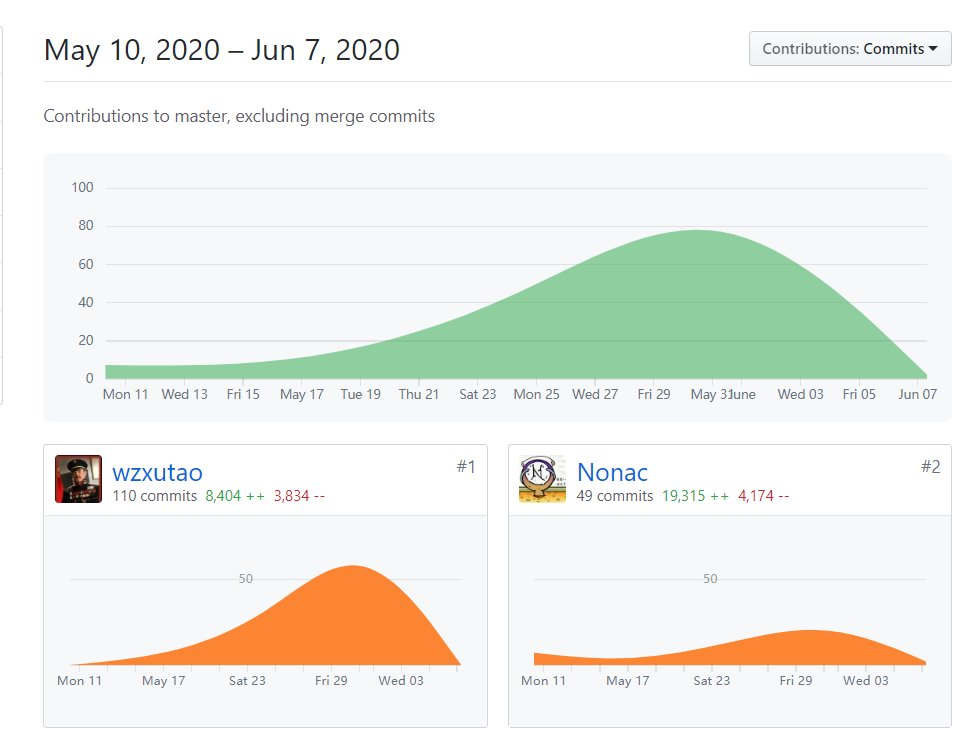
\includegraphics[scale=0.7]{figures/github.png}
		\caption{After Effect}
		\label{fig:15}
	\end{figure}
	
	% --------------------
	
\end{spacing}	
	
\end{document}